\chapter{Variational Perspective: From VAEs to DDPMs}\label{ch:variational}


In this chapter we view diffusion models through a variational lens. We begin with the Variational Autoencoders (VAEs), which represent data with latent variables and are trained by maximizing a tractable lower bound on the log likelihood. In this setting a learned encoder maps observations to latents, and a learned decoder maps latents back to observations, closing the modeling loop. 

Building on this pattern, hierarchical variants (Hierarchical VAEs) stack several latent layers to capture structure at multiple scales. With this setup, Denoising Diffusion Probabilistic Models (DDPM) follow the same template: instead of jointly training both the encoder and decoder, the encoder is fixed as a forward noising process that gradually maps data to noise, and training learns a decoder that reverses this path in successive denoising steps. In this view, VAEs, hierarchical VAEs, and diffusion models all optimize a likelihood surrogate defined by a variational bound, providing a common foundation for the methods introduced here.





\newpage
\section{Variational Autoencoder}\label{sec:vae}
How can a neural network learn to generate realistic data?  
A natural starting point is the \emph{autoencoder}, which consists of two networks:  
a deterministic \emph{encoder} that compresses an input to a low-dimensional latent code, and a deterministic \emph{decoder} that reconstructs the input from this code.  
Training minimizes the reconstruction error between the original input and its reconstruction.  
While this setup enables accurate reconstruction, the latent space is unstructured: randomly sampling latent codes usually produces meaningless outputs, limiting the model’s use for generation.



% How can a neural network learn to generate realistic data? A natural starting point is the autoencoder, a framework \se{introduce networks (encoder, decoder) first, then discuss how they are trained} trained to reconstruct inputs through a low dimensional latent representation. A deterministic encoder compresses the input into a latent code, which a deterministic decoder then uses to reconstruct the original data. While this setup enables faithful reconstruction, it lacks a structured latent space. As a result, decoding randomly sampled latent codes typically yields meaningless outputs, making the model ineffective for generation.

The \emph{Variational Autoencoder (VAE)} \citep{kingma2013auto}  solves this by imposing a probabilistic structure on the latent space. This transforms the model from a simple reconstruction tool into a true generative model, capable of producing novel and realistic data.



\subsection{Probabilistic Encoder and Decoder}

\begin{figure}[tbh!]
\centering
\resizebox{0.85\linewidth}{!}{%
\begin{tikzpicture}[>=Latex, thick, font=\sffamily, node distance=0.8cm]

\tikzset{
  state/.style={
    rectangle, rounded corners=3pt,
    draw=black, fill=gray!10,
    minimum height=45pt, minimum width=25pt, align=center,
    % Add outer sep to ensure arrows connect cleanly to the rounded edges
    outer sep=0pt 
  },
  latent/.style={
    rectangle, rounded corners=3pt,
    draw=black, fill=gray!10,
    minimum height=28pt, minimum width=28pt, align=center,
    outer sep=0pt
  },
  encoderblock/.style={
    trapezium, trapezium stretches=true,
    % Adjust angles to create the frustum shape.
    % The 'top' and 'bottom' here refer to the sides that become the vertical parallels after rotation.
    trapezium left angle=80,  % Closer to 90 for less slope
    trapezium right angle=80, % Closer to 90 for less slope
    shape border rotate=270,   % Rotate 90 degrees clockwise for vertical parallels
    draw=black, fill=gray!20,
    minimum height=8pt, minimum width=15pt, inner sep=4pt, align=center
  },
  decoderblock/.style={
    trapezium, trapezium stretches=true,
    trapezium left angle=80,
    trapezium right angle=80,
    shape border rotate=90,  % Rotate 270 degrees clockwise (or -90)
    draw=black, fill=gray!20,
    minimum height=8pt, minimum width=15pt, inner sep=4pt, align=center
  }
}

% nodes
\node[state] (x) {$\mathbf{x}$};
\node[encoderblock, right=of x] (enc) {\footnotesize\textbf{Encoder}\\[-2pt]
 \footnotesize $q_{\bm{\theta}}(\mathbf{z}|\mathbf{x})$}; % Using bm for bold math
\node[latent, right=of enc] (z) {$\mathbf{z}$};
\node[decoderblock, right=of z] (dec) {\footnotesize\textbf{Decoder}\\[-2pt]
  \footnotesize$p_{\bm{\phi}}(\mathbf{x}|\mathbf{z})$}; % Using bm for bold math
\node[state, right=of dec] (xprime) {$\mathbf{x}'$};

% short arrows (edge-to-edge)
\draw[->] (x) -- (enc); % Changed to direct node-to-node, TikZ usually finds the nearest edge
\draw[->] (enc) -- (z);
\draw[->] (z) -- (dec);
\draw[->] (dec) -- (xprime);

\end{tikzpicture}}
\caption{\textbfs{Illustration of a VAE.} It consists of a stochastic encoder $q_{\bm{\theta}}(\rvz|\rvx)$ that maps data $\rvx$ to a latent variable $\rvz$, and a decoder $p_{\bm{\phi}}(\rvx|\rvz)$ that reconstructs data from the latent. \figcredit{Created by the authors.}}
\label{fig:vae-graph}
\end{figure}

\paragraph{Construction of Decoder (Generator).}

% Our objective is to model the data generation process. VAE assumes that each observation $\mathbf{x}$ is generated from a latent variable $\mathbf{z}$ drawn from a simple \emph{prior distribution}, typically standard Gaussian: $\mathbf{z} \sim p_{\text{prior}} := \mathcal{N}(\mathbf{0}, \mathbf{I})$. More precisely, we define a \emph{decoder (generator)} network $p_{\bm{\phi}}(\mathbf{x}|\mathbf{z})$, which learns to generate data from latent inputs $\rvz$. New samples are generated by first sampling $\mathbf{z} \sim p_{\text{prior}}$ and then decoding via $\mathbf{x} \sim p_{\bm{\phi}}(\mathbf{x}|\mathbf{z})$.

% \se{need to say the decoder is simple, like a gaussian or fully factor. also probably give some intuition? maybe something along the lines that generating pixels is hard, but it becomes easier if we have a bunch of features (latent vars) that describe content, colors, etc}

% The VAE defines a latent-variable generative model via the marginal likelihood:
% \[
% p_{\bm{\phi}}(\mathbf{x}) = \int p_{\bm{\phi}}(\mathbf{x}|\mathbf{z}) p(\mathbf{z}) \mathrm{d}\mathbf{z}.
% \]
% Ideally, the decoder parameters $\bm{\phi}$ would be learned by maximizing the marginal likelihood of the observed data, as in maximum likelihood training (see \Cref{eq:MLE}). However, this objective is generally intractable for expressive, non-linear decoders, since the marginalization over latent variables $\mathbf{z}$ lacks a closed-form solution. As a result, direct MLE becomes computationally infeasible.
In VAEs, we distinguish between two types of variables: 
\emph{observed variables} $\rvx$, which correspond to the data we see (e.g., an image), 
and \emph{latent variables} $\rvz$, which capture the hidden factors of variation 
(e.g., object shape, color, or style). 
The model assumes that each observation $\rvx$ is generated from a latent variable 
sampled from a simple \emph{prior distribution}, typically a standard Gaussian, 
$\rvz \sim p_{\text{prior}} := \mathcal{N}(\mathbf{0}, \mathbf{I})$.

To map $\rvz$ back to data space, we define a \emph{decoder (generator)} distribution 
$p_{\bm{\phi}}(\rvx|\rvz)$. In practice, this decoder is kept simple, often a 
factorized Gaussian (see \Cref{subsec:optimization-vae}) or similar distribution, so that learning focuses on extracting 
useful latent features rather than memorizing data. 
Intuitively, directly generating pixels one by one is extremely hard; instead, the 
latent variable provides a compact representation, 
from which decoding the exact pixel arrangement becomes much easier. 
New samples are drawn by first sampling $\rvz \sim p_{\text{prior}}$ and then 
decoding via $\rvx \sim p_{\bm{\phi}}(\rvx|\rvz)$.

The VAE thereby defines a latent-variable generative model through the marginal likelihood:
\[
p_{\bm{\phi}}(\rvx) = \int p_{\bm{\phi}}(\rvx|\rvz) p(\rvz) \diff \rvz.
\]
Ideally, the decoder parameters $\bm{\phi}$ are learned by maximizing this marginal 
likelihood, as in maximum likelihood estimation (see \Cref{eq:MLE}). 
However, because the integral over $\rvz$ is intractable for expressive, non-linear 
decoders, direct MLE is computationally infeasible, motivating the variational 
approach used in VAEs.

% \se{i think you need to use some text to clearly explain the difference between observed and latent vars at the beginning}



\paragraph{Construction of Encoder (Inference Network).}
% To get a handle on our intractable generator, we might try to reverse the process: given a real data point $\mathbf{x}$, what distribution of latent codes $\mathbf{z}$ could have been its origin? The formal answer is given by Bayes' rule:
% \[
% p_{\bm{\phi}}(\mathbf{z}|\mathbf{x}) = \frac{p_{\bm{\phi}}(\mathbf{x}|\mathbf{z})p(\mathbf{z})}{p_{\bm{\phi}}(\mathbf{x})}.
% \]
% But this brings us to a second, related impasse. The denominator is $p_{\bm{\phi}}(\mathbf{x})$, the very intractable likelihood that halted our progress in the first place. We are in a computational catch: to train our generator, we need to solve an inference problem that itself requires a trained generator. \se{this is confusing. the generator doesn't have to be trained.}

% This is where the ``variational'' in VAE makes its brilliant entrance. \se{brilliant is inappropriate. keep scientific language as dry/objective as possible}
% Instead of calculating this ideal mapping exactly, we learn to \emph{approximate} it. We introduce a second neural network, the \emph{encoder} $q_{\bm{\theta}}(\mathbf{z}|\mathbf{x})$, and give it a crucial job: act as a tractable and learnable proxy for the intractable true mapping.
% \[
% q_{\bm{\theta}}(\mathbf{z}|\mathbf{x}) \approx p_{\bm{\phi}}(\mathbf{z}|\mathbf{x}).
% \]
% This encoder  takes in real data and outputs a distribution over the latent space, providing the essential, workable link from $\mathbf{x}$ back to $\mathbf{z}$ that we need to build our objective. \se{wording is a bit odd}


To connect our intractable generator to real data, consider the reverse question:  
given an observation $\rvx$, what latent codes $\rvz$ could have produced it?  
By Bayes’ rule, the posterior distribution is
\[
p_{\bm{\phi}}(\rvz|\rvx) \;=\; \frac{p_{\bm{\phi}}(\rvx|\rvz) p(\rvz)}{p_{\bm{\phi}}(\rvx)}.
\]
The difficulty is that the denominator involves the marginal likelihood $p_{\bm{\phi}}(\rvx)$,  
which requires integrating over all latent variables and is intractable for nonlinear decoders.  
Thus, exact inference of $\rvz$ from $\rvx$ is computationally prohibitive.

The ``variational'' step in VAEs addresses this by replacing the intractable posterior with a tractable approximation.  
We introduce an \emph{encoder} (or inference network) $q_{\bm{\theta}}(\rvz|\rvx)$, parameterized by a neural network,  
whose role is to serve as a learnable proxy:
\[
q_{\bm{\theta}}(\rvz|\rvx) \;\approx\; p_{\bm{\phi}}(\rvz|\rvx).
\]
In practice, the encoder maps each observed data point $\rvx$ to a distribution over latent codes,  
providing a feasible and trainable pathway from $\rvx$ back to $\rvz$ that enables learning.




\subsection{Training via the Evidence Lower Bound (ELBO)}

We now define a computable training objective. While we cannot directly optimize $\log p_{\bm{\phi}}(\mathbf{x})$, we can maximize a lower bound on it—the \emph{Evidence Lower Bound (ELBO)}:

\thmp{Evidence Lower Bound (ELBO)}{elbo}{
For any data point $\mathbf{x}$, the log-likelihood satisfies:
\[
\log p_{\bm{\phi}}(\mathbf{x}) \geq \mathcal{L}_{\text{ELBO}}(\bm{\theta}, \bm{\phi}; \mathbf{x}),
\]
where the ELBO is given by: 
\begin{align}\label{eq:vae-elbo}
    \mathcal{L}_{\text{ELBO}} = \underbrace{\mathbb{E}_{\mathbf{z} \sim q_{\bm{\theta}}(\mathbf{z}|\mathbf{x})} \left[ \log p_{\bm{\phi}}(\mathbf{x}|\mathbf{z}) \right]}_{\text{Reconstruction Term}} - \underbrace{\mathcal{D}_{\mathrm{KL}}\left( q_{\bm{\theta}}(\mathbf{z}|\mathbf{x}) \| p(\mathbf{z}) \right)}_{\text{Latent Regularization}}.
\end{align}
}{
The ELBO arises from Jensen’s inequality:
\begin{align*}
\log p_{\bm{\phi}}(\mathbf{x}) &= \log \int p_{\bm{\phi}}(\mathbf{x}, \mathbf{z})   \mathrm{d}\mathbf{z} = \log \int q_{\bm{\theta}}(\mathbf{z}|\mathbf{x}) \frac{p_{\bm{\phi}}(\mathbf{x}, \mathbf{z})}{q_{\bm{\theta}}(\mathbf{z}|\mathbf{x})}   \mathrm{d}\mathbf{z} \\
&= \log \mathbb{E}_{\mathbf{z} \sim q_{\bm{\theta}}(\mathbf{z}|\mathbf{x})} \left[ \frac{p_{\bm{\phi}}(\mathbf{x}, \mathbf{z})}{q_{\bm{\theta}}(\mathbf{z}|\mathbf{x})} \right] \geq \mathbb{E}_{\mathbf{z} \sim q_{\bm{\theta}}(\mathbf{z}|\mathbf{x})} \left[ \log \frac{p_{\bm{\phi}}(\mathbf{x}, \mathbf{z})}{q_{\bm{\theta}}(\mathbf{z}|\mathbf{x})} \right].
\end{align*}
}
The ELBO objective naturally decomposes into two parts:
\begin{itemize}
    % \item \textbfs{Reconstruction:} Encourages accurate reconstruction of $\mathbf{x}$ from $\mathbf{z}$. This objective arises naturally from a KL-based variational inequality. However, on its own, it merely memorizes the training data, motivating a second KL term to regularize the latent space for generative modeling.
    % \se{refer back to the  earlier autoencoder discussion}
    \item \textbfs{Reconstruction:} Encourages accurate recovery of $\mathbf{x}$ from its latent code $\mathbf{z}$. With Gaussian encoder and decoder assumptions, this term reduces exactly to the familiar reconstruction loss of an autoencoder (cf.\ \Cref{subsec:optimization-vae}). However, as in autoencoders, optimizing this term alone risks memorizing the training data, motivating an additional regularization.
    \item \textbfs{Latent KL:} Encourages the encoder distribution $q_{\bm{\theta}}(\mathbf{z}|\mathbf{x})$ to stay close to a simple Gaussian prior $p_{\mathrm{prior}}(\mathbf{z})$. This regularization shapes the latent space into a smooth and continuous structure, enabling meaningful generation by ensuring that samples drawn from the prior can be reliably decoded.
\end{itemize}
This trade-off ensures both faithful reconstructions and coherent sampling.

\paragraph{Information-Theoretic View: ELBO as a Divergence Bound.}
% The ELBO objective enjoys a deep connection to information theory. To understand this, we recall that MLE training is equivalent to minimizing the KL divergence
% \[
% \mathcal{D}_{\mathrm{KL}}(p_{\text{data}}(\rvx) \| p_{\bm{\phi}}(\rvx)),
% \]
% which measures how well the generative model approximates the true data distribution. However, this quantity is generally intractable. The variational framework offers a powerful workaround by introducing a joint comparison.

% Let us consider the two joint distributions induced by the decoder and the encoder:
% \begin{itemize}
%     \item The \textbfs{generative joint}, $p_{\bm{\phi}}(\mathbf{x}, \mathbf{z}) = p(\mathbf{z}) p_{\bm{\phi}}(\mathbf{x}|\mathbf{z})$, which represents the model’s generative process.
%     \item The \textbfs{inference joint}, $q_{\bm{\theta}}(\mathbf{x}, \mathbf{z}) = p_{\text{data}}(\mathbf{x}) q_{\bm{\theta}}(\mathbf{z}|\mathbf{x})$, which couples real data with its encoded latent.
% \end{itemize}
% Comparing these joints gives rise to the inequality
% \begin{align}\label{eq:joint-bound}
%     \mathcal{D}_{\mathrm{KL}}(p_{\text{data}}(\rvx) \| p_{\bm{\phi}}(\rvx)) \leq \mathcal{D}_{\mathrm{KL}}(q_{\bm{\theta}}(\mathbf{x}, \mathbf{z}) \| p_{\bm{\phi}}(\mathbf{x}, \mathbf{z})),
% \end{align}
% % \se{notations are a bit inconsistent (sometimes with arguments, sometimes not)}
% which follows from the \emph{Data Processing Inequality (DPI)} and is also known as the ``chain rule for KL divergence''. The intuition is that marginalizing the latent cause $\mathbf{z}$ to observe only the outcome $\mathbf{x}$ can obscure modeling discrepancies that are only revealed when comparing the full joint processes.
% \se{the DPI story doesn't seem fitting to me, it's usually in terms of mutual information}

% To make this precise, observe the decomposition:
% \begin{align*}
%     &\underbrace{\mathcal{D}_{\mathrm{KL}}(q_{\bm{\theta}}(\mathbf{x}, \mathbf{z}) \| p_{\bm{\phi}}(\mathbf{x}, \mathbf{z}))}_{\text{Total Error Bound}} 
%     \\=& \mathbb{E}_{q_{\bm{\theta}}(\mathbf{x}, \mathbf{z})} \left[ \log \frac{p_{\text{data}}(\mathbf{x}) q_{\bm{\theta}}(\mathbf{z}|\mathbf{x})}{p_{\bm{\phi}}(\mathbf{x}) p_{\bm{\phi}}(\mathbf{z}|\mathbf{x})} \right] \\=&\mathbb{E}_{p_{\text{data}}(\mathbf{x})} \left[ \log \frac{p_{\text{data}}(\mathbf{x})}{p_{\bm{\phi}}(\mathbf{x})} + \mathcal{D}_{\mathrm{KL}}\left( q_{\bm{\theta}}(\mathbf{z}|\mathbf{x}) \| p_{\bm{\phi}}(\mathbf{z}|\mathbf{x}) \right) \right] \\
%     \\=&  \underbrace{\mathcal{D}_{\mathrm{KL}}(p_{\text{data}} \| p_{\bm{\phi}})}_{\text{True Modeling Error}} + \underbrace{\mathbb{E}_{p_{\text{data}}(\mathbf{x})} \big[ \mathcal{D}_{\mathrm{KL}}( q_{\bm{\theta}}(\mathbf{z}|\mathbf{x}) \| p_{\bm{\phi}}(\mathbf{z}|\mathbf{x}) ) \big]}_{\text{Inference Error}}.
% \end{align*}
% This identity yields a valuable interpretation: the joint KL divergence decomposes into the marginal KL of interest and the expected discrepancy between the approximate and true posteriors. The latter is always non-negative, confirming the DPI.

% Moreover, observe that
% \[
% \log p_{\bm{\phi}}(\mathbf{x}) - \mathcal{L}_{\text{ELBO}}(\bm{\theta}, \bm{\phi}; \mathbf{x}) = \mathcal{D}_{\mathrm{KL}}\left( q_{\bm{\theta}}(\mathbf{z}|\mathbf{x}) \| p_{\bm{\phi}}(\mathbf{z}|\mathbf{x}) \right),
% \]
% so the ``inference error'' term corresponds precisely to the gap between the true log-likelihood and the ELBO. Therefore, when we train a VAE by maximizing the ELBO, we are explicitly minimizing the inference error. This shows that our practical training algorithm is directly optimizing a meaningful component of the overall information-theoretic bound on how well our model captures the true data distribution.



% \se{you could consider adding a mixture of gaussians (discrete latent) as an example too to build intuition for the mixture effect}



The ELBO objective has a natural information-theoretic interpretation. 
Recall that maximum likelihood training amounts to minimizing the KL divergence
\[
\mathcal{D}_{\mathrm{KL}}(p_{\text{data}}(\rvx) \| p_{\bm{\phi}}(\rvx)),
\]
which measures how well the model distribution approximates the data distribution. 
Since this term is intractable in general, the variational framework introduces a joint comparison.

Specifically, consider two joint distributions:
\begin{itemize}
    \item The \textbfs{generative joint}, $p_{\bm{\phi}}(\rvx, \rvz) = p(\rvz) p_{\bm{\phi}}(\rvx|\rvz)$, which describes how the model generates data;
    \item The \textbfs{inference joint}, $q_{\bm{\theta}}(\rvx, \rvz) = p_{\text{data}}(\rvx) q_{\bm{\theta}}(\rvz|\rvx)$, which couples real data with its inferred latent.
\end{itemize}
Comparing these distributions yields the inequality
\begin{align}\label{eq:joint-bound}
    \mathcal{D}_{\mathrm{KL}}(p_{\text{data}}(\rvx) \| p_{\bm{\phi}}(\rvx)) 
    \leq \mathcal{D}_{\mathrm{KL}}(q_{\bm{\theta}}(\rvx,\rvz) \| p_{\bm{\phi}}(\rvx,\rvz)),
\end{align}
sometimes referred to as the chain rule for KL divergence. 
Intuitively, comparing only marginals ($\rvx$) can hide mismatches that are revealed when the full latent–data joint is considered.

Formally, one can expand the joint KL as
\begin{align*}
    &\underbrace{\mathcal{D}_{\mathrm{KL}}(q_{\bm{\theta}}(\mathbf{x}, \mathbf{z}) \| p_{\bm{\phi}}(\mathbf{x}, \mathbf{z}))}_{\text{Total Error Bound}} 
    \\=& \mathbb{E}_{q_{\bm{\theta}}(\mathbf{x}, \mathbf{z})} \left[ \log \frac{p_{\text{data}}(\mathbf{x}) q_{\bm{\theta}}(\mathbf{z}|\mathbf{x})}{p_{\bm{\phi}}(\mathbf{x}) p_{\bm{\phi}}(\mathbf{z}|\mathbf{x})} \right] \\=&\mathbb{E}_{p_{\text{data}}(\mathbf{x})} \left[ \log \frac{p_{\text{data}}(\mathbf{x})}{p_{\bm{\phi}}(\mathbf{x})} + \mathcal{D}_{\mathrm{KL}}\left( q_{\bm{\theta}}(\mathbf{z}|\mathbf{x}) \| p_{\bm{\phi}}(\mathbf{z}|\mathbf{x}) \right) \right] \\
    \\=&  \underbrace{\mathcal{D}_{\mathrm{KL}}(p_{\text{data}} \| p_{\bm{\phi}})}_{\text{True Modeling Error}} + \underbrace{\mathbb{E}_{p_{\text{data}}(\mathbf{x})} \big[ \mathcal{D}_{\mathrm{KL}}( q_{\bm{\theta}}(\mathbf{z}|\mathbf{x}) \| p_{\bm{\phi}}(\mathbf{z}|\mathbf{x}) ) \big]}_{\text{Inference Error}},
\end{align*}
where the first term is the true modeling error and the second is the inference error, i.e., the gap between the approximate and true posteriors. The latter is always non-negative, which explains \Cref{eq:joint-bound}.

Finally, note that
\[
\log p_{\bm{\phi}}(\rvx) - \mathcal{L}_{\text{ELBO}}(\bm{\theta},\bm{\phi};\rvx) 
= \mathcal{D}_{\mathrm{KL}} \left(q_{\bm{\theta}}(\rvz|\rvx)\|p_{\bm{\phi}}(\rvz|\rvx)\right).
\]
Thus the inference error is exactly the gap between the log-likelihood and the ELBO. 
Maximizing the ELBO therefore corresponds to directly reducing inference error, ensuring that training minimizes a meaningful part of the overall bound.



% \se{you could consider adding a mixture of gaussians (discrete latent) as an example too to build intuition for the mixture effect}



% \begin{figure}
%     \begin{center}
% \scalebox{0.8}{
% \begin{tikzpicture}[node distance=3cm and 4cm, auto, >=Stealth]

% % Nodes
% \node[draw, rounded corners, minimum height=1.3cm, minimum width=4cm] (minKL) 
%     {$\displaystyle \min_{\bm{\phi}} \mathcal{D}(p_{\text{data}} \| p_{\bm{\phi}}) $};
% \node[draw, rounded corners, minimum height=1.3cm, minimum width=5cm, right=of minKL] (maxLogLik) 
%     {$\displaystyle \max_{\bm{\phi}} \mathbb{E}_{p_{\text{data}}}[\log p_{\bm{\phi}}]$};

% \node[draw, rounded corners, minimum height=1.3cm, minimum width=4cm, below=2.5cm of minKL] (minJointKL)
%     {$\displaystyle \min_{\bm{\phi},\bm{\theta}} \mathcal{D}\big(q_{\bm{\theta}}(\rvx,\rvz) \| p_{\bm{\phi}}(\rvx,\rvz)\big)$};
% \node[draw, rounded corners, minimum height=1.3cm, minimum width=4cm, right=of minJointKL] (maxELBO) 
%     {$\displaystyle \max_{\bm{\phi},\bm{\theta}} \mathbb{E}_{p_{\text{data}}} \big[ \mathcal{L}_{\mathrm{ELBO}}(\theta,\phi; \rvx) \big]$};

% % Arrows and labels
% \draw[<->, thick] (minKL) -- (maxLogLik) node[midway, above]{ \Cref{eq:MLE}};
% \draw[<->, thick] (minJointKL) -- (maxELBO) node[midway, above]{ \Cref{eq:joint-elbo}};

% % Vertical connectors
% \draw[thick] ($(minKL.south) + (0,0)$) -- ($(minJointKL.north) + (0,0)$);
% \draw[thick] ($(maxLogLik.south) + (0,0)$) -- ($(maxELBO.north) + (0,0)$);

% % Vertical labels
% \node at ($(minKL)!0.5!(minJointKL)$) [left=0.3cm] {\parbox{2cm}{\centering Theorem 2.1.1 \\ \rotatebox{270}{\Large$\leq$}}};
% \node at ($(maxLogLik)!0.5!(maxELBO)$) [right=0.3cm] {\parbox{2cm}{\centering Theorem 2.1.2 \\ \rotatebox{270}{\Large$\leq$}}};

% \end{tikzpicture}
% }
% \end{center}
%     \caption{Relations between marginal KL minimization and likelihood maximization (top) and their tractable upper-bound joint latent-variable counterparts with ELBO (bottom).
% }
% \label{fig:elbo-joint}
% \end{figure}


\subsection{Gaussian VAE}\label{subsec:optimization-vae}
A standard formulation of the VAE employs Gaussian distributions for both the encoder and decoder.
\paragraph{Encoder Part.}
The encoder $ q_{\bm{\theta}}(\mathbf{z} | \mathbf{x}) $ is typically modeled as a Gaussian distribution as:
\[
q_{\bm{\theta}}(\mathbf{z} | \mathbf{x}) := \mathcal{N}\left(\mathbf{z}; \bm{\mu}_{\bm{\theta}}(\mathbf{x}), \operatorname{diag}(\bm{\sigma}_{\bm{\theta}}^2(\mathbf{x}))\right),
\]
where $\bm{\mu}_{\bm{\theta}} : \mathbb{R}^D \to \mathbb{R}^d$ and $\bm{\sigma}_{\bm{\theta}} : \mathbb{R}^D \to \mathbb{R}_+^d$ are deterministic outputs of the encoder network.
\paragraph{Decoder Part.} The decoder is typically modeled as a Gaussian distribution with fixed variance:
\[
p_{\bm{\phi}}(\mathbf{x}|\mathbf{z}) := \mathcal{N}\bigl(\mathbf{x}; \bm{\mu}_{\bm{\phi}}(\mathbf{z}), \sigma^2 \rmI\bigr),
\]
where $\bm{\mu}_{\bm{\phi}} : \mathbb{R}^d \to \mathbb{R}^D$ is a neural network, and $\sigma > 0$ is a small constant controlling the variance.
 
Under this assumption, the reconstruction term in the ELBO simplifies as
\[
\mathbb{E}_{q_{\bm{\theta}}(\mathbf{z} | \mathbf{x})} \left[\log p_{\bm{\phi}}(\mathbf{x} | \mathbf{z})\right]
= - \frac{1}{2\sigma^2} \mathbb{E}_{q_{\bm{\theta}}(\mathbf{z} | \mathbf{x})} \left[\|\mathbf{x} - \bm{\mu}_{\bm{\phi}}(\mathbf{z})\|^2\right] + C,
\]
where $C$ is a constant independent of $\bm{\theta}$ and $\bm{\phi}$. The ELBO objective thus reduces to:
\[
\min_{\bm{\theta}, \bm{\phi}}  \mathbb{E}_{q_{\bm{\theta}}(\mathbf{z} | \mathbf{x})} \left[ \frac{1}{2\sigma^2} \|\mathbf{x} - \bm{\mu}_{\bm{\phi}}(\mathbf{z})\|^2 \right]
+ \mathcal{D}_{\mathrm{KL}}\big(q_{\bm{\theta}}(\mathbf{z} | \mathbf{x}) \| p_{\mathrm{prior}}(\mathbf{z})\big),
\]
where the KL term admits a closed-form solution due to the Gaussian assumption. Training the VAE therefore reduces to minimizing a regularized reconstruction loss.

\subsection{Drawbacks of Standard VAE}\label{sec:drawback_standard_VAE}
Despite the theoretical appeal of the VAE framework, it suffers from a critical drawback: it often produces blurry outputs.

\paragraph{Blurry Generations in VAEs.}
To understand this phenomenon, consider a fixed Gaussian encoder $ q_{\text{enc}}(\mathbf{z}|\mathbf{x}) $, and a decoder of the form
\[
p_{\text{dec}}(\mathbf{x}|\mathbf{z}) = \mathcal{N}(\mathbf{x}; \bm{\mu}(\rvz), \sigma^2 \rmI),
\]
where $ \bm{\mu}(\rvz) $ denotes the decoder network. With an arbitrary encoder, optimizing the ELBO reduces (up to an additive constant) to minimizing the expected reconstruction error:
\[
\argmin_{\bm{\mu}} \mathbb{E}_{p_{\text{data}}(\mathbf{x})q_{\text{enc}}(\mathbf{z}|\mathbf{x})} \left[ \| \mathbf{x} - \bm{\mu}(\rvz) \|^2 \right].
\]
This is a standard least squares problem in $ \bm{\mu}(\rvz) $, and its solution is given in closed form by the conditional mean:
\[
\bm{\mu}^*(\mathbf{z}) = \mathbb{E}_{q_{\text{enc}}(\mathbf{x}|\mathbf{z})}[\mathbf{x}],
\]
where $ q_{\text{enc}}(\mathbf{x}|\mathbf{z}) $ is the encoder-induced posterior on inputs given latents, defined via Bayes’ rule:
\[
q_{\text{enc}}(\mathbf{x}|\mathbf{z})
=
\frac{q_{\text{enc}}(\mathbf{z}|\mathbf{x})\, p_{\text{data}}(\mathbf{x})}{q_{\text{enc}}(\mathbf{z})},
\qquad
q_{\text{enc}}(\mathbf{z})
:=
\int q_{\text{enc}}(\mathbf{z}|\mathbf{x})\, p_{\text{data}}(\mathbf{x})\, \diff \mathbf{x}.
\]

An equivalent form of the optimal generator via Bayes' rule is:
\[
\bm{\mu}^*(\mathbf{z})
=
\frac{\mathbb{E}_{p_{\text{data}}(\mathbf{x})}\!\left[q_{\text{enc}}(\mathbf{z}|\mathbf{x}) \cdot \mathbf{x}\right]}
{q_{\text{enc}}(\mathbf{z})}
=
\frac{\mathbb{E}_{p_{\text{data}}(\mathbf{x})}\!\left[q_{\text{enc}}(\mathbf{z}|\mathbf{x}) \cdot \mathbf{x}\right]}
{\mathbb{E}_{p_{\text{data}}(\mathbf{x})}\!\left[q_{\text{enc}}(\mathbf{z}|\mathbf{x})\right]}.
\]
Now suppose that two distinct inputs $ \mathbf{x} \neq \mathbf{x}' $ are mapped to overlapping regions in latent space, i.e., the supports of $ q_{\text{enc}}(\cdot|\mathbf{x}) $ and $ q_{\text{enc}}(\cdot|\mathbf{x}') $ intersect. Then $\bm{\mu}^*(\mathbf{z})$ averages over multiple, potentially unrelated inputs, which leads to blurry, non-distinct outputs. This averaging effect over conflicting modes is a fundamental reason for the characteristic blurriness in VAE-generated samples.




\newpage
\subsection{(Optional) From Standard VAE to Hierarchical VAEs}
To model complex data, Hierarchical Variational Autoencoders (HVAEs)
\citep{vahdat2020nvae} enhance VAEs by introducing a hierarchy of latent variables. This deep, layered structure allows the model to capture data features at multiple levels of abstraction, significantly boosting expressive power and mirroring the compositional nature of real-world data.
\vspace{0.3cm}
\begin{figure}[tbh!]
    \centering
\begin{tikzpicture}[
    ->, % Sets default arrow type
    >=Stealth, % Sets default arrowhead style
    node_dist/.style={right=1.7cm of #1}, % Style for node distance
    font=\small,
    thick
  ]

  % Define a style for the circular nodes
  \tikzset{state/.style={
      rectangle,
      rounded corners=3pt,
      draw=black,
      fill=gray!10,
      minimum height=35pt,
      minimum width=25pt
    }
  }

  % Place the nodes
  \node[state] (x) {$\rvx$};
  \node[state] (z1) [node_dist=x] {$\rvz_1$};
  \node[state] (z2) [node_dist=z1] {$\rvz_2$};
  \node (dots) [right=0.7cm of z2] {$\boldsymbol{\cdots}$};
  \node[state] (zT) [node_dist=dots] {$\rvz_L$};

  % Draw the arrows (edges) with labels
  
  % Inference path (top, q, forward) - Shifted up
  \path ([yshift=4.5pt]x.east)  edge node[above] {$q_{\bm{\theta}}(\rvz_1|\rvx)$} ([yshift=4.5pt]z1.west);
  \path ([yshift=4.5pt]z1.east) edge node[above] {$q_{\bm{\theta}}(\rvz_2|\rvz_1)$} ([yshift=4.5pt]z2.west);
  \path ([yshift=4.5pt]z2.east) edge ([yshift=4.5pt]dots.west);
  % --- CHANGED: Added pos=0.4 to shift label left ---
  \path ([yshift=4.5pt]dots.east) edge node[above, pos=0.4] {$q_{\bm{\theta}}(\rvz_L|\rvz_{L-1})$} ([yshift=4.5pt]zT.west);
  
  % Generative path (bottom, p, backward) - Shifted down
  \path ([yshift=-4.5pt]z1.west) edge node[below] {$p_{\bm{\phi}}(\rvx|\rvz_1)$} ([yshift=-4.5pt]x.east);
  \path ([yshift=-4.5pt]z2.west) edge node[below] {$p_{\bm{\phi}}(\rvz_1|\rvz_2)$} ([yshift=-4.5pt]z1.east);
  \path ([yshift=-4.5pt]dots.west) edge ([yshift=-4.5pt]z2.east);
  % --- CHANGED: Added pos=0.6 to shift label left ---
  \path ([yshift=-4.5pt]zT.west) edge node[below, pos=0.6] {$p_{\bm{\phi}}(\rvz_{L-1}|\rvz_L)$} ([yshift=-4.5pt]dots.east);

\end{tikzpicture}

    \caption{\textbfs{Computation graph of the HVAE.} It has a hierarchical structure with stacked, trainable encoders and decoders across multiple latent layers. \figcredit{Created by the authors.}
}
    \label{fig:hvae-graph}
\end{figure}


\paragraph{HVAE's Modeling.}
Unlike standard VAEs that use a single latent code $\mathbf{z}$, hierarchical VAEs (HVAEs) introduce multiple layers of latent variables arranged in a top-down hierarchy.  
Each latent layer conditions the one below it, forming a chain of conditional priors that captures structure at progressively finer levels of abstraction.  
This leads to the following top-down factorization of the joint distribution:

% :
% \[
% p_{\bm{\phi}}(\mathbf{x}|\mathbf{z}_1) \leftarrow p_{\bm{\phi}}(\mathbf{z}_1|\mathbf{z}_2) \leftarrow \ldots \leftarrow p_{\bm{\phi}}(\mathbf{z}_{L-1}|\mathbf{z}_L) \leftarrow p(\mathbf{z}_L) =: p_{\text{prior}},
% \]
% \se{messy and imprecise notation, i would remove this}
\[
p_{\bm{\phi}}(\mathbf{x}, \mathbf{z}_{1:L}) = p_{\bm{\phi}}(\mathbf{x} | \mathbf{z}_1) \prod_{i=2}^{L} p_{\bm{\phi}}(\mathbf{z}_{i-1}|\mathbf{z}_i)   p(\mathbf{z}_L).
\]
This structure defines the marginal data distribution,
\[
p_{\text{HVAE}}(\mathbf{x}) := \int p_{\bm{\phi}}(\mathbf{x}, \mathbf{z}_{1:L}) \diff \mathbf{z}_{1:L}.
\]
 Generation proceeds progressively: starting from the top latent variable $ \mathbf{z}_L $, each latent is decoded sequentially down to $ \mathbf{z}_1 $, followed by generating the final observation $ \mathbf{x} $.

For encoding part, HVAEs utilize a structured, learnable variational encoder $ q_{\bm{\theta}}(\mathbf{z}_{1:L}|\mathbf{x}) $ that mirrors the generative hierarchy. A common choice is a bottom-up Markov factorization:
\[
q_{\bm{\theta}}(\mathbf{z}_{1:L} | \mathbf{x}) = q_{\bm{\theta}}(\mathbf{z}_1 | \mathbf{x}) \prod_{i=2}^{L} q_{\bm{\theta}}(\mathbf{z}_i | \mathbf{z}_{i-1}).
\]

\paragraph{HVAE's ELBO.}
Similar to \Cref{eq:vae-elbo}, ELBO is derived via Jensen's inequality:
\begin{align}\label{eq:hvae-elbo}
\begin{aligned}
    \log p_{\text{HVAE}}(\mathbf{x}) 
&= \log \int p_{\bm{\phi}}(\mathbf{x}, \mathbf{z}_{1:L}) \diff \mathbf{z}_{1:L} \\
&= \log \int \frac{p_{\bm{\phi}}(\mathbf{x}, \mathbf{z}_{1:L})}{q_{\bm{\theta}}(\mathbf{z}_{1:L}|\mathbf{x})}   q_{\bm{\theta}}(\mathbf{z}_{1:L}|\mathbf{x}) \diff \mathbf{z}_{1:L} \\
&= \log \mathbb{E}_{q_{\bm{\theta}}(\mathbf{z}_{1:L}|\mathbf{x})} \left[ \frac{p_{\bm{\phi}}(\mathbf{x}, \mathbf{z}_{1:L})}{q_{\bm{\theta}}(\mathbf{z}_{1:L}|\mathbf{x})} \right] \\
&\geq \mathbb{E}_{q_{\bm{\theta}}(\mathbf{z}_{1:L}|\mathbf{x})} \left[ \log \frac{p_{\bm{\phi}}(\mathbf{x}, \mathbf{z}_{1:L})}{q_{\bm{\theta}}(\mathbf{z}_{1:L}|\mathbf{x})} \right]\\
&=:\mathcal{L}_{\text{ELBO}}(\bm{\phi}).
\end{aligned}
\end{align}
Substituting the factorized forms yields:
\begin{align*}
\mathcal{L}_{\text{ELBO}} 
= \mathbb{E}_{q_{\bm{\theta}}(\mathbf{z}_{1:L}|\mathbf{x})} \left[ 
\log \frac{
p(\mathbf{z}_L) \prod_{i=2}^{L} p_{\bm{\phi}}(\mathbf{z}_{i-1} | \mathbf{z}_i)   p_{\bm{\phi}}(\mathbf{x} | \mathbf{z}_1)
}{
q_{\bm{\theta}}(\mathbf{z}_1|\mathbf{x}) \prod_{i=2}^{L} q_{\bm{\theta}}(\mathbf{z}_i|\mathbf{z}_{i-1})
}
\right].
\end{align*}

This hierarchical ELBO decomposes into interpretable terms, including a
reconstruction term, adjacent-layer matching terms, and a top-level KL
regularizer to the prior.

The leap from shallow to deep networks revolutionized machine learning, and a similar idea transformed generative models. HVAEs showed the power of using deep, stacked layers to build data. This concept of a layered hierarchy is a cornerstone of modern generative modeling, appearing again in score-based methods (\Cref{sec:SMLD}) and normalizing flows (\Cref{sec:flow-based-method}). The core insight is simple yet powerful: 
\msg{Observation}{}{Stacking layers allows the model to generate data progressively, starting with coarse details and adding finer ones at each step. This process makes it far easier to capture the complex structure of high-dimensional data.}

% \se{readers might wonder why not just make the neural net deeper. might be worth explaining}




\paragraph{Why Deeper Networks in a Flat VAE are Not Enough.} There are two fundamental limitations of a standard flat VAE that are not resolved by simply making the encoder and decoder deeper.


The first limitation is the variational family. In a standard VAE,
\[
q_\btheta(\rvz| \rvx)=\mathcal N \big(\rvz;\,\bm{\mu}_{\btheta}(\rvx), \operatorname{diag}(\sigma_\theta^2(\rvx))\big),
\]
so for each fixed $\rvx$ the encoder posterior is a single Gaussian with diagonal
covariance. Greater network depth improves the accuracy of $\bm{\mu}_{\btheta}$ and
$\sigma_\btheta$ but does not expand the family; even a full covariance remains
one unimodal ellipsoid. When $p_\bphi(\rvz| \rvx)$ is multi-peaked, this family cannot match it, which loosens the ELBO and
weakens inference. Addressing this requires a richer posterior class, not merely deeper networks.


Second, if the decoder is too expressive, the model may suffer from posterior collapse. To see why, let us recall that the objective of the VAE is
\begin{align*}
&\mathbb{E}_{p_{\text{data}}(\mathbf{x})}[\mathcal L_{\mathrm{ELBO}}(\rvx)]\\
&\quad\quad=\E_{p_{\text{data}}(\mathbf{x})q_\btheta(\rvz|\rvx)}[\log p_\bphi(\rvx|\rvz)]
-\mathbb{E}_{p_{\text{data}}(\mathbf{x})}\big[\mathcal{D}_\mathrm{KL} \big(q_\btheta(\rvz|\rvx) \| p(\rvz)\big)\big]\\
&\quad\quad=\E_{p_{\text{data}}(\mathbf{x})q_\btheta(\rvz|\rvx)}[\log p_\bphi(\rvx|\rvz)]-\mathcal I_q(\rvx;\rvz) - \mathcal{D}_\mathrm{KL}(q_{\bm{\theta}}(\rvz) \| p(\rvz)),
\end{align*}
where $\mathcal I_q(\rvx;\rvz)$ is the mutual information defined by
\[
\mathcal I_q(\rvx;\rvz)
=\E_{q(\rvx,\rvz)} \Big[\log \tfrac{q_\btheta(\rvz|\rvx)}{q(\rvz)}\Big]
=\E_{p_{\mathrm{data}}(\rvx)} \big[\mathcal{D}_\mathrm{KL}(q_\btheta(\rvz|\rvx) \| q(\rvz))\big],
\]
and the aggregated posterior is $q_{\bm{\theta}}(\rvz)= \int p_{\mathrm{data}}(\rvx) q_\btheta(\rvz|\rvx) \diff\rvx$.

If the decoder class can model the data well without using $\rvz$ (i.e., it contains some $p_\bphi(\rvx|\rvz)=r(\rvx)$ close to $p_{\mathrm{data}}$), then a maximizer of the ELBO sets $q_\btheta(\rvz|\rvx)=p(\rvz)$, so $\mathcal I_q(\rvx;\rvz)=0$ and $q_\btheta(\rvz)=p(\rvz)$. This ``ignore $\rvz$'' solution does not disappear by making the networks deeper: (1) the learned code becomes independent of $\rvx$ (so it carries no data-dependent structure useful for downstream tasks), and (2) conditioning or moving in $\rvz$ has no effect on generated samples, so controllable generation fails.


\paragraph{What Hierarchy Changes?}
An HVAE introduces multiple latent levels,
\[
p_\bphi(\rvx,\rvz_{1:L})=p_\bphi(\rvx|\rvz_1)\prod_{i=2}^L p_\bphi(\rvz_{i-1}|\rvz_i) p(\rvz_L),
\]
with ELBO
\begin{align*}
\mathcal L_{\mathrm{ELBO}}(\rvx)
&= \E_{q_\btheta(\rvz_1|\rvx)}[\log p_\bphi(\rvx|\rvz_1)]
\\
&\quad - \E_{q_\btheta(\rvz_{1:2}|\rvx)}
\big[\log q_\btheta(\rvz_1|\rvx)-\log p_\bphi(\rvz_1|\rvz_2)\big]
\\
&\quad - \sum_{i=2}^{L-1}
\E_{q_\btheta(\rvz_{1:i+1}|\rvx)}
\big[\log q_\btheta(\rvz_i|\rvz_{i-1})-\log p_\bphi(\rvz_i|\rvz_{i+1})\big]
\\
&\quad - \E_{q_\btheta(\rvz_{L-1}|\rvx)}
\Big[\mathcal{D}_{\mathrm{KL}}(q_\btheta(\rvz_L|\rvz_{L-1}) \| p(\rvz_L))\Big].
\end{align*}
Here, we denote $\E_q := \E_{p_{\mathrm{data}}(\rvx) q_{\btheta}(\rvz_{1:L}|\rvx)}$.
Each latent level interacts only with its neighboring levels in the
hierarchy: the encoder passes information upward through
$q_\btheta(\rvz_i|\rvz_{i-1})$, while the decoder passes information
downward through $p_\bphi(\rvz_{i-1}|\rvz_i)$. Accordingly, the ELBO
decomposes into a reconstruction term, adjacent-layer matching terms,
and a top-level KL regularizer to the prior. These properties stem from
the hierarchical latent graph, not from simply deepening networks in a
flat VAE.

\paragraph{What Will be Ahead?}
While HVAEs extend the VAE framework with multiple latent layers for expressiveness, their training poses unique challenges. Because the encoder and decoder must be optimized jointly, learning becomes unstable: lower layers and the decoder can already reconstruct $\rvx$, leaving higher-level latents with little effective signal. Moreover, gradient information reaching deeper variables is often indirect and weak, making it difficult for them to contribute meaningfully. An additional difficulty lies in balancing model capacity, since overly expressive conditionals  can dominate the reconstruction task and suppress the utility of higher latents. 


Interestingly, the core idea of a deep, layered hierarchy finds a more powerful incarnation in variational diffusion models, a topic we explore in \Cref{sec:ddpm}. Diffusion models inherit the progressive structure of HVAEs but elegantly sidestep their central weakness. By fixing the encoding process and focusing solely on learning the generative reversal, they unlock newfound stability and modeling flexibility, leading to a significant leap in the quality of generated outputs.

For notational simplicity, we deviate from the common VAE convention that uses $q$ for the encoder and $p$ for the generator. To avoid ambiguity, we denote distributions as 
$p$ and will always specify their roles through appropriate subscripts or superscripts, clarifying them in context.


% For notational consistency throughout this work, we will deviate from the common VAE convention that distinguishes the encoder ($q$) from the generator ($p$). Hereafter, we will use the symbol $p$ to refer to distributions in both the inference and generative processes. \jcc{We will rely on context, along with specific subscripts or superscripts, to unambiguously define the role of each distribution.}
% \se{this seems dangerous..} 
% \jcc{i'll check for later chapters to see if we should change the notation for $q$. for instance, I'm using $p_t$ $p_{\mathrm{data}}$ everywhere after DDPM..., especially, aligning Score SDE notations.}





% \begin{table}[th]
%   \caption{Summary of the trade-off between KL divergence and reconstruction in VAEs. 
% }
%   \small
%   \centering
%   \resizebox{\textwidth}{!}{
%   \begin{tabular}{ccccc}
%      \toprule
%         & \textbfs{Encoder Behavior} & \textbfs{KL Term} & \textbfs{Recon. Quality} & \textbfs{Gen. Quality} \\
%      \midrule
%     Perfect KL 
%       & Posterior = Prior 
%       & $\downarrow$ 
%       & Poor
%       & \begin{tabular}{@{}c@{}} Posterior collapse: \\ uninformative latent,  blurry samples \end{tabular} \\
%     Perfect Recon. 
%       & Posterior far from Prior 
%       & $\uparrow$ 
%       & Good
%       & \begin{tabular}{@{}c@{}}  Prior hole problem: \\ poor generation from $p_{\text{prior}}$  \end{tabular} \\
%      \bottomrule
%   \end{tabular}
%   }
%   \label{tb:vae-kl-recon-tradeoff}
% \end{table}


% \emph{Posterior collapse} occurs when the approximate posterior matches the prior:
% \[
% q_{\bm{\phi}}(\mathbf{z}|\mathbf{x}) \approx p(\mathbf{z}),
% \]
% causing $\mathbf{z}$ to carry little information about $\mathbf{x}$ and yielding uninformative, blurry samples.
% The \emph{prior hole problem} arises when the aggregated posterior
% \[
% q_{\bm{\phi}}(\mathbf{z}) = \int q_{\bm{\phi}}(\mathbf{z}|\mathbf{x}) p_{\mathrm{data}}(\mathbf{x})  \diff\mathbf{x}
% \]
% covers only part of the prior support, leaving some latent regions unvisited during training. The decoder is then poorly trained in these regions, resulting in low-quality samples from latent codes sampled there.

\clearpage
\newpage
%%%%%

\section{Variational Perspective: DDPM}\label{sec:ddpm}

Denoising Diffusion Probabilistic Models (DDPMs) \citep{sohl2015deep,ho2020denoising} represent a cornerstone of diffusion modeling. Conceptually, they operate within a variational framework, much like VAEs and HVAEs. However, DDPMs introduce a clever twist that tackles some of the challenges faced by their predecessors.

At their core, DDPMs involve two distinct stochastic processes:
\begin{itemize}
    \item \textbfs{The Forward Pass (Fixed Encoder):} This process gradually corrupts data by injecting Gaussian noise over multiple steps via a transition kernel $p(\mathbf{x}_{i}|\mathbf{x}_{i-1})$. The data evolves into an isotropic Gaussian distribution, effectively becoming pure noise. This means the encoder is fixed and not learned.
    \item \textbfs{The Reverse Denoising Process (Learnable Decoder):} Here, a neural network learns to reverse the noise corruption through a parameterized distribution $p_{\bm{\phi}}(\mathbf{x}_{i-1}|\mathbf{x}_{i})$. Starting from pure noise, this process iteratively denoises to generate realistic samples. Crucially, each individual denoising step is a more manageable task than generating a complete sample from scratch, as VAEs often attempt to do.
\end{itemize}
By fixing the encoder and concentrating learning on the gradual generative trajectory, DDPMs achieve remarkable stability and expressive power. 

\vspace{0.3cm}
\begin{figure}[tbh!]
    \centering
\begin{tikzpicture}[
    ->, % Sets default arrow type
    >=Stealth, % Sets default arrowhead style
    node_dist/.style={right=1.7cm of #1}, % Style for node distance
    font=\small,
    thick
  ]

  % Define a style for the nodes
  \tikzset{state/.style={
      rectangle,
      rounded corners=3pt,
      draw=black,
      fill=gray!10, % Made the node fill lighter
      minimum height=35pt,
      minimum width=25pt
    }
  }

  % Place the nodes
  \node[state] (x) {$\rvx_0$};
  \node[state] (z1) [node_dist=x] {$\rvx_1$};
  \node[state] (z2) [node_dist=z1] {$\rvx_2$};
  \node (dots) [right=0.7cm of z2] {$\boldsymbol{\cdots}$};
  \node[state] (zT) [node_dist=dots] {$\rvx_L$};

  % Draw the arrows (edges) with labels
  
  % Inference path (top, q, forward) - Shifted up
  % Changed 'darkgray' to 'gray' for a lighter color
  \path [gray] ([yshift=4.5pt]x.east)  edge node[above] {$p(\rvx_1|\rvx_0)$} ([yshift=4.5pt]z1.west);
  \path [gray] ([yshift=4.5pt]z1.east) edge node[above] {$p(\rvx_2|\rvx_1)$} ([yshift=4.5pt]z2.west);
  \path [gray] ([yshift=4.5pt]z2.east) edge ([yshift=4.5pt]dots.west);
  \path [gray] ([yshift=4.5pt]dots.east) edge node[above, pos=0.4] {$p(\rvx_L|\rvx_{L-1})$} ([yshift=4.5pt]zT.west);
  
  % Generative path (bottom, p, backward) - Shifted down
  \path ([yshift=-4.5pt]z1.west) edge node[below] {$p_{\bm{\phi}}(\rvx_0|\rvx_1)$} ([yshift=-4.5pt]x.east);
  \path ([yshift=-4.5pt]z2.west) edge node[below] {$p_{\bm{\phi}}(\rvx_1|\rvx_2)$} ([yshift=-4.5pt]z1.east);
  \path ([yshift=-4.5pt]dots.west) edge ([yshift=-4.5pt]z2.east);
  \path ([yshift=-4.5pt]zT.west) edge node[below, pos=0.6] {$p_{\bm{\phi}}(\rvx_{L-1}|\rvx_L)$} ([yshift=-4.5pt]dots.east);

\end{tikzpicture}
    \caption{\textbfs{Illustration of DDPM.} It consists of a fixed forward process (in gray) that gradually adds Gaussian noise to the data, and a learned reverse process that denoises step-by-step to generate new samples. \figcredit{Created by the authors.}}
     \label{fig:vdm-grap}
\end{figure}


% \begin{figure}[th!]
%     \centering
%     \includegraphics[width=\linewidth]{Images/PartB/vdm-graph.pdf}
%     \caption{Illustration of DDPM. It consists of a fixed forward process that gradually adds Gaussian noise to the data, and a learned reverse process that denoises step-by-step to generate new samples.}
%     \label{fig:vdm-graph}
% \end{figure}

In this section, we focus on DDPMs, postponing the broader discussion to \Cref{sec:variational-perspective}, where we present a more general and flexible framework.


\subsection{Forward Process (Fixed Encoder)}
In DDPMs, the forward process is a fixed, non-trainable operation that serves as an encoder. It progressively corrupts the original data by adding noise over multiple steps, eventually transforming it into a simple prior distribution $p_{\text{prior}} := \mathcal{N}(\mathbf{0}, \mathbf{I})$. This transformation is depicted as the forward chain in \Cref{fig:vdm-grap} or as illustrated in \Cref{fig:vdm-forward}.

\begin{figure}[tbh!]
    \centering
    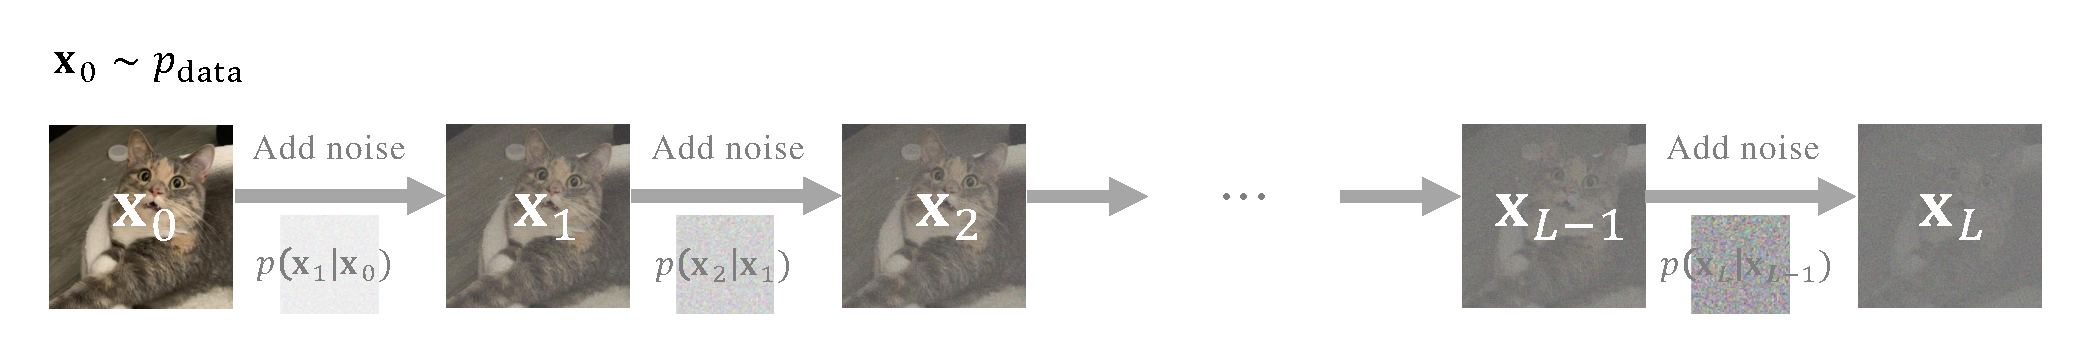
\includegraphics[width=\linewidth]{Images/PartB/vdm-forward.pdf}
    \caption{Illustration of the DDPM forward process, wherein Gaussian noise is incrementally added to corrupt a data sample into pure noise. \figcredit{Created by the authors.}}
    \label{fig:vdm-forward}
\end{figure}

% \se{check indexing ranges below (from 0 or 1), seems off by one}

Let us formalize this step-by-step degradation:
\paragraph{Fixed Gaussian Transitions.}
Each step in the forward process is governed by a fixed Gaussian transition kernel\footnote{This formulation, while potentially appearing different, is mathematically equivalent to the original DDPM transition kernel.}:
\[
p(\rvx_i|\rvx_{i-1}) := \mathcal{N}(\rvx_i; \sqrt{1 - \beta_i^2}   \rvx_{i-1}, \beta_i^2 \rmI).
\]
Here, the process begins with $\rvx_{0} $, representing a sample drawn from the real data distribution $p_{\text{data}}$. The sequence $\{\beta_i\}_{i=1}^L$ denotes a pre-determined, monotonically increasing noise schedule, where each 
$\beta_i \in (0, 1)$ controls the variance of the Gaussian noise injected at step $i$.  For convenience, we define $\alpha_i := \sqrt{1 - \beta_i^2}$. This mathematical definition is precisely equivalent to the following intuitive iterative update:
\[
\rvx_i = \alpha_i \rvx_{i-1} + \beta_i \bm{\epsilon}_i,  
\]
where $\bm{\epsilon}_i \sim \mathcal{N}(\bm{0}, \rmI)$ are independently and identically distributed. This means at each step $i$, we scale down the previous state $\rvx_{i-1}$ by $\alpha_i$ and add a controlled amount of Gaussian noise scaled by $\beta_i$.

\paragraph{Perturbation Kernel and Prior Distribution.}
By recursively applying the transition kernels, we obtain a closed-form expression for the distribution of noisy samples at step $i$ given the original data $\rvx_0$:
\[
p_i(\rvx_i|\rvx_0) = \mathcal{N}\left(\rvx_i; \bar{\alpha}_i \rvx_0, (1 - \bar{\alpha}_i^2) \rmI \right),
\]
where 
\[
\bar{\alpha}_i := \prod_{k=1}^i \sqrt{1-\beta_k^2} = \prod_{k=1}^i \alpha_k.
\]
This means we can sample $\rvx_i$ directly from $\rvx$ as
\begin{align}\label{eq:ddpm-forward}
    \rvx_i = \bar{\alpha}_i \rvx_0 + \sqrt{1-\bar{\alpha}_i^2}   \bm{\epsilon}, \quad \bm{\epsilon} \sim \mathcal{N}(\bm{0}, \rmI).
\end{align}
Let the noise schedule $ \{\beta_i\}_{i=1}^L $ be an increasing sequence, then the marginal distribution of the forward process converges as
\[
p_L(\mathbf{x}_L | \rvx_0) \longrightarrow \mathcal{N}(\mathbf{0}, \mathbf{I}) \quad \text{as } L \to \infty,
\]
which motivates the choice of the prior distribution as
\[
p_{\text{prior}} := \mathcal{N}(\mathbf{0}, \mathbf{I})
\]
with no reliance on data $\rvx_0$.
% \paragraph{Marginal Densities.}
% By marginalizing over the data distribution using the law of total probability, the marginal density at step $i$ is
% \[
% p_i(\rvx_i) := \int p_i(\rvx_i|\rvx) p_{\text{data}}(\rvx_0) \diff \rvx_0.
% \]
% \se{what's the point of this paragraph?}


\subsection{Reverse Denoising Process (Learnable Decoder)}

% \se{this section packs too much content, too many formulas and will be overwhelming. since it is important, you need to break it up more and more gradually} \jcc{I cut the original section into 3 subsections: one is about oracle $p(\rvx_{i-1}|\rvx_i)$ and introduce high-level idea; the next subsection is about how to model $p_\bphi(\rvx_{i-1}|\rvx_i)$ with practical losses/parametrizations introduced there (\S 2.2.3); and the last one is Practical Choices of Predictions and Loss (\S 2.2.4). Also, I added some bridging and intuition.}

At its core, the essence of DDPMs lies in their ability to \emph{reverse} the controlled degradation imposed by the forward diffusion process. Starting from pure, unstructured noise, $\mathbf{x}_L \sim p_{\text{prior}}$, the objective is to progressively \emph{denoise} this randomness, step by step, until a coherent and meaningful data sample emerges. This reverse generation proceeds through a Markov chain, illustrated by \Cref{fig:ddpm-sampling-formal-rev}.
\begin{figure}[tbh!]
    \centering
    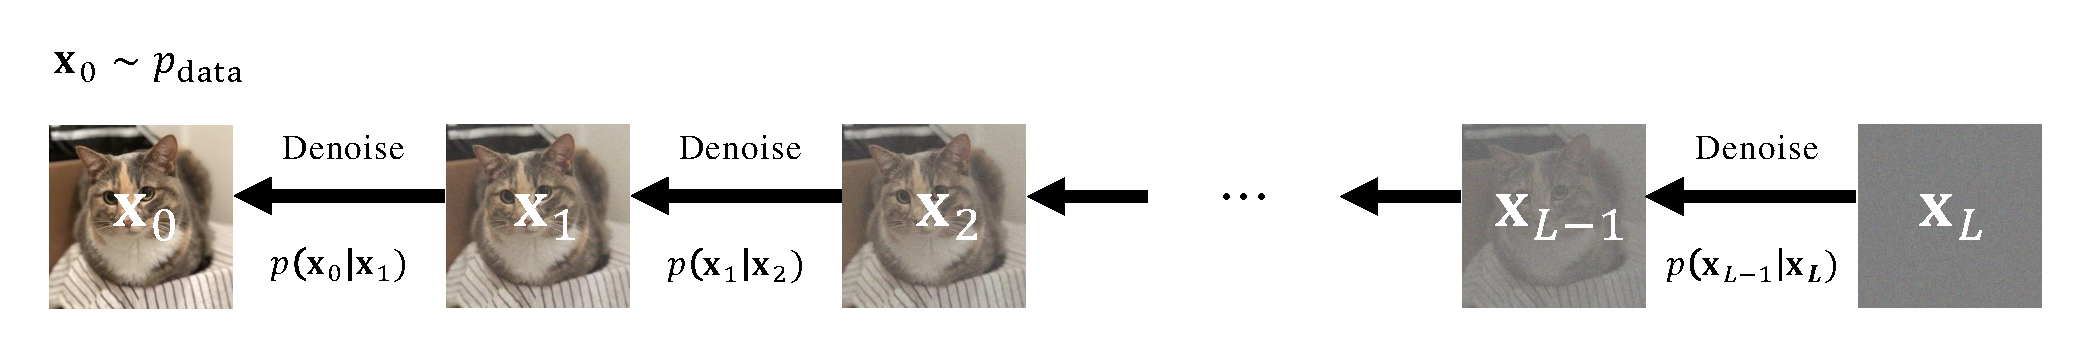
\includegraphics[width=\linewidth]{Images/PartB/vdm-backward.pdf}
\caption{\textbfs{Illustration of DDPM reverse (denoising) process.} Starting from noise $\mathbf{x}_L \sim  p_{\mathrm{prior}}$, the model sequentially samples $\mathbf{x}_{i-1} \sim  p(\mathbf{x}_{i-1}|\mathbf{x}_i)$ for $i=L,\ldots,1$ to obtain a newly generated data $\mathbf{x}_0$. The oracle transition $p(\mathbf{x}_{i-1}|\mathbf{x}_i)$ is unknown; thus, we aim to approximate it.
\figcredit{Created by the authors.}
}

    \label{fig:ddpm-sampling-formal-rev}
\end{figure}





The fundamental challenge, and the central question guiding DDPM development, then becomes:
\begin{question}
Can we precisely compute, or at least effectively approximate, these reverse transition kernels $ p(\mathbf{x}_{i-1}|\mathbf{x}_i) $, especially when considering the complex distribution of $\mathbf{x}_i \sim p_i(\mathbf{x}_i)$?
\end{question}

Rather than diving immediately into the mathematically intricate derivation of the Evidence Lower Bound (ELBO), as the original DDPM paper does (for which a detailed discussion awaits in \Cref{subsec:ddpm-elbo}), we will instead approach the training objective from a more intuitive perspective: by leveraging conditional probabilities to achieve a tractable formulation. 


\paragraph{Overview: Modeling and Training Objective.} 
To enable the generative process, our goal is to approximate the unknown true reverse transition kernel, $p(\mathbf{x}_{i-1}|\mathbf{x}_i)$. We achieve this by introducing a learnable parametric model, $p_{\bm{\phi}}(\mathbf{x}_{i-1}|\mathbf{x}_i)$, and training it to minimize the expected KL divergence:
\begin{align}\label{eq:marginal-kl-matching}
    \mathbb{E}_{p_i(\mathbf{x}_i)} \left[
    \mathcal{D}_{\mathrm{KL}}\big(p(\mathbf{x}_{i-1}|\mathbf{x}_i) \| p_{\bm{\phi}}(\mathbf{x}_{i-1}|\mathbf{x}_i)\big)
    \right].
\end{align}

However, a direct computation of the target distribution $p(\mathbf{x}_{i-1}|\mathbf{x}_i)$ is challenging. By Bayes' theorem, we would need to evaluate:
\[
p(\mathbf{x}_{i-1}|\mathbf{x}_i) = p(\mathbf{x}_i|\mathbf{x}_{i-1}) \underbrace{\frac{p_{i-1}(\mathbf{x}_{i-1})}{p_i(\mathbf{x}_i)}}_{\text{intractable}}.
\]
The marginals $p_i(\rvx_i)$ and $p_{i-1}(\rvx_{i-1})$ are expectations over the unknown data distribution $p_{\mathrm{data}}$, given by:
\[
p_i(\rvx_i) = \int p_i(\rvx_i | \rvx_0) p_{\mathrm{data}}(\rvx_0) \mathrm{d}\rvx_0,
\]
and analogously for $p_{i-1}(\rvx_{i-1})$. Since $p_{\mathrm{data}}$ is unknown, these integrals have no closed-form evaluation; at best they can be approximated from samples, so the exact densities are not available in practice.

\begin{figure}[th!]
    \centering
    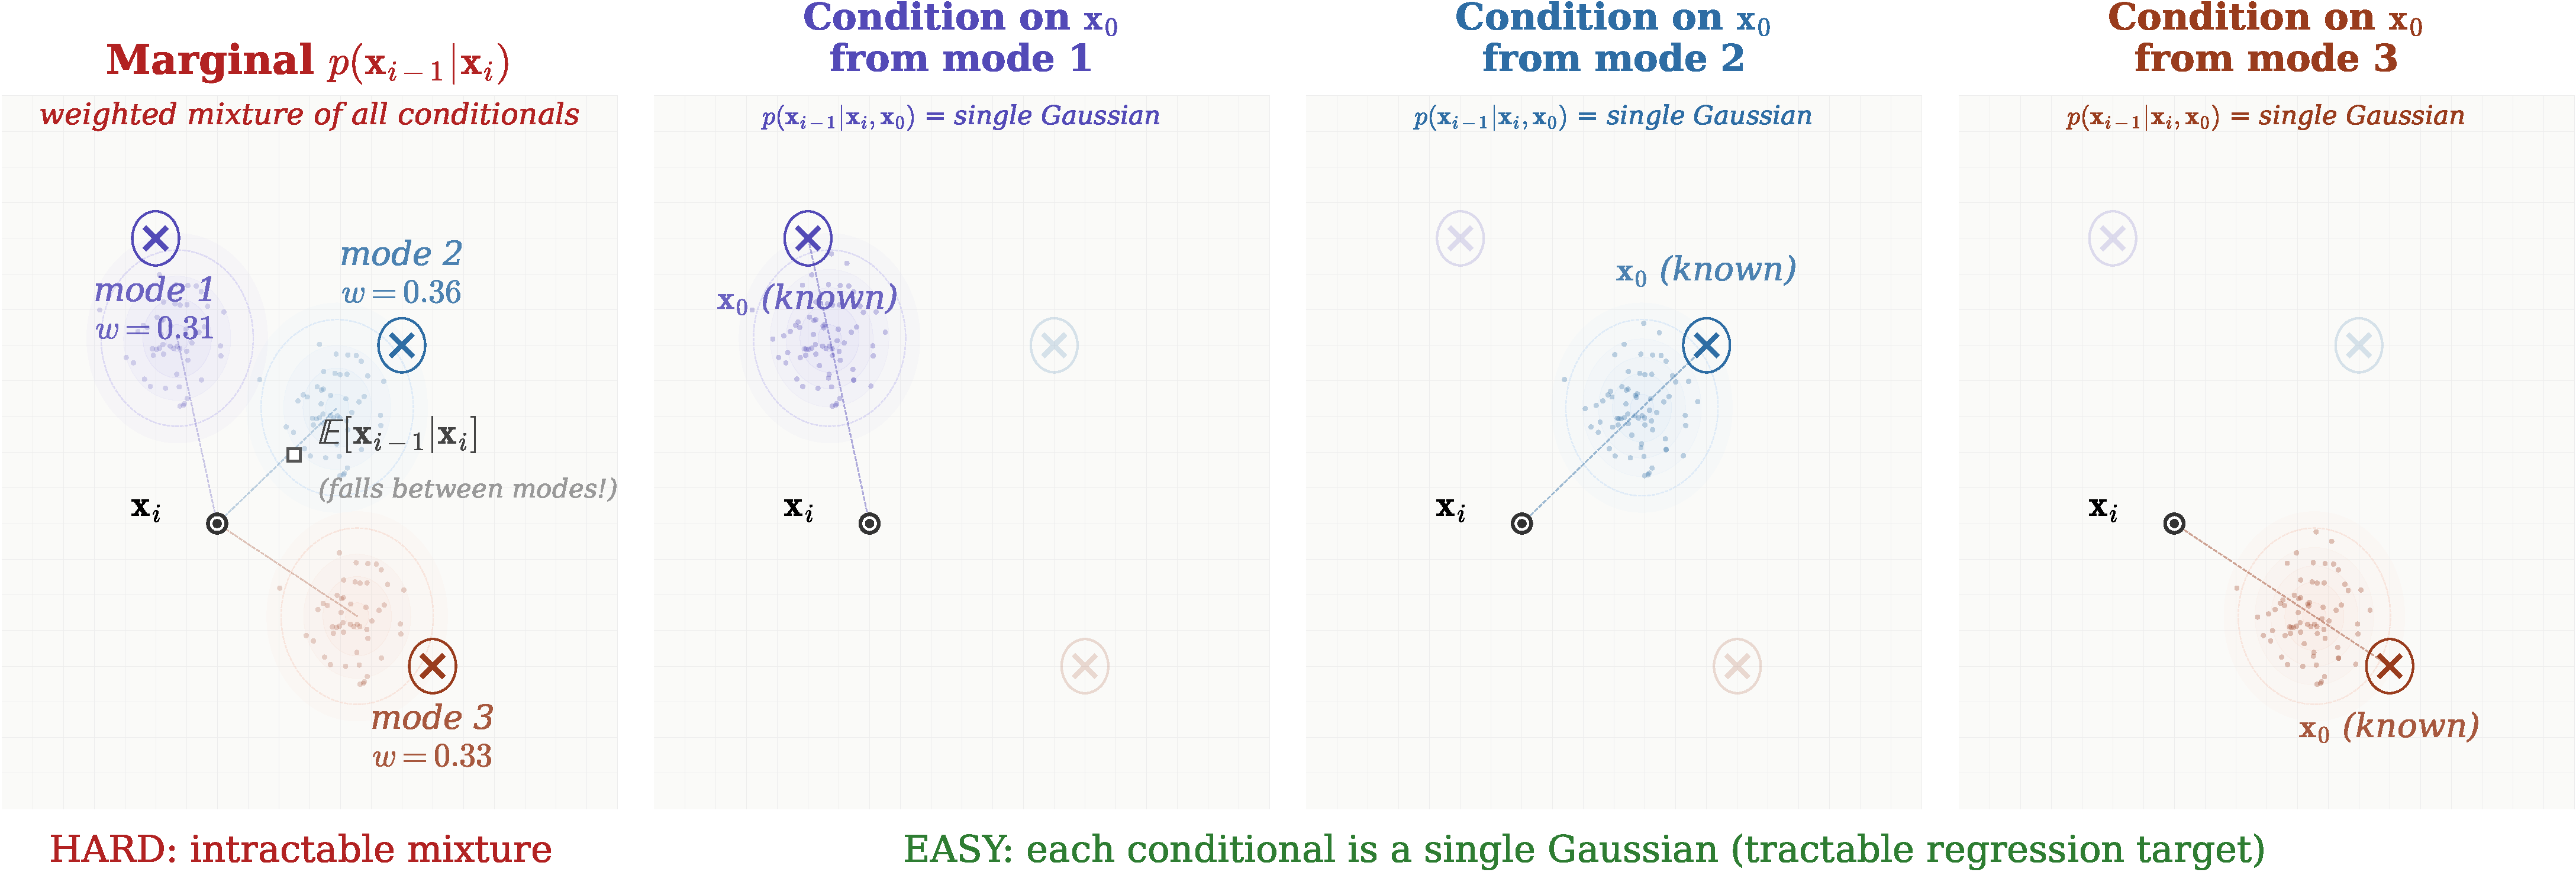
\includegraphics[width=\linewidth]{Images/PartB/ddpm_conditional_trick.pdf}
    \caption{\textbfs{Illustration of the conditioning trick in DDPM.}
For a fixed noisy sample $\rvx_i$, the true reverse distribution
$p(\rvx_{i-1}|\rvx_i)$ is induced by marginalizing over all possible clean origins $\rvx_0$, and is therefore generally a mixture that can be multimodal.
Its mean may even fall between modes, making direct prediction difficult.
By contrast, once we condition on the clean sample $\rvx_0$, the reverse posterior
$p(\rvx_{i-1}|\rvx_i,\rvx_0)$ becomes a single Gaussian.
DDPM exploits this tractable conditional structure during training, replacing a difficult multimodal prediction problem with a tractable regression target. \figcredit{Created by the authors with AI-assisted coding.}}
    \label{fig:conditional-trick}
\end{figure}


\paragraph{Overcoming Intractability with Conditioning.}
A central insight in DDPMs resolves this intractability: we condition the reverse transition on a clean data sample $\mathbf{x}_0$. This subtle yet powerful step transforms the intractable kernel into one that is mathematically tractable:
\[
p(\mathbf{x}_{i-1}|\mathbf{x}_i, \mathbf{x}_0) = p(\mathbf{x}_i|\mathbf{x}_{i-1}) \frac{p(\mathbf{x}_{i-1}|\mathbf{x}_0)}{p(\mathbf{x}_i|\mathbf{x}_0)}.
\]
This tractability arises from two key properties of the forward process: its Markov property, meaning $p(\mathbf{x}_i|\mathbf{x}_{i-1}, \mathbf{x}_0) = p(\mathbf{x}_i|\mathbf{x}_{i-1})$, and the Gaussian nature of all involved distributions. As a result, $p(\mathbf{x}_{i-1}|\mathbf{x}_i, \mathbf{x}_0)$ itself is Gaussian and admits a closed-form expression (which we will see in \Cref{eq:ddpm-reverse-mean}). We visualize it in \Cref{fig:conditional-trick}. Crucially, this elegant conditioning strategy allows us to derive a tractable objective that is functionally equivalent to the seemingly intractable marginal KL divergence in \Cref{eq:marginal-kl-matching}.

\thmp{Equivalence Between Marginal and Conditional KL Minimization}{equiv-marginal-kl}{
The following equality holds:
\begin{align}\label{eq:kl-matching}
\begin{aligned}
    &\mathbb{E}_{p_i(\rvx_i)}\left[
        \mathcal{D}_{\mathrm{KL}}\big(p(\rvx_{i-1}|\rvx_i) \| p_{\bm{\phi}}(\rvx_{i-1}|\rvx_i)\big)
    \right] \\
    ={}&
    \mathbb{E}_{p_{\mathrm{data}}(\rvx_0)}
    \mathbb{E}_{p(\rvx_i|\rvx_0)} \left[
        \mathcal{D}_{\mathrm{KL}}\big(p(\rvx_{i-1}|\rvx_i, \rvx_0) \| p_{\bm{\phi}}(\rvx_{i-1}|\rvx_i)\big)
    \right] + C.
\end{aligned}
\end{align}
where $C$ is a constant independent of $\bm{\phi}$. Moreover, the minimizer of \Cref{eq:kl-matching} satisfies
\[
p^*(\mathbf{x}_{i-1}|\mathbf{x}_i) = \mathbb{E}_{p(\mathbf{x}_0|\mathbf{x}_i)} \big[p(\mathbf{x}_{i-1}|\mathbf{x}_i, \mathbf{x}_0)\big] = p(\mathbf{x}_{i-1}|\mathbf{x}_i), \quad \mathbf{x}_i \sim p_i.
\]
}{The proof rewrites a KL-divergence expectation by expanding definitions, applying the chain rule of probability, and using a logarithmic identity to decompose it into the sum of an expected conditional KL divergence and a marginal KL divergence. A complete derivation is in \Cref{subsec:proof-equiv-marginal-kl}.}


This alternative viewpoint: conditioning to obtain a tractable objective, forms the foundation of DDPMs and reveals a profound commonality with other influential diffusion models, as we will explore in \Cref{ch:score-based} and \Cref{ch:flow-based}.


It reveals a powerful equivalence: minimizing the KL divergence between marginal distributions is mathematically identical to minimizing the KL divergence between specific conditional distributions. This latter formulation is exceptionally useful because the crucial conditional distribution, $p(\mathbf{x}_{i-1}|\mathbf{x}_i, \mathbf{x})$, possesses a convenient closed-form expression:
\lem{Reverse Conditional Transition Kernel}{ddpm-reverse-kernel}{$p(\mathbf{x}_{i-1} | \mathbf{x}_i, \mathbf{x})$ is Gaussian with the closed-form expression:
\begin{align*}
    p(\rvx_{i-1} | \rvx_i, \rvx) =\mathcal{N}\left(\rvx_{i-1}; \bm{\mu}\left(\rvx_i, \rvx, i\right), \sigma^2(i)\rmI \right),
\end{align*}
where
\begin{align}\label{eq:ddpm-reverse-mean}
\begin{aligned}
            \bm{\mu}\left(\rvx_i, \rvx, i\right):= \frac{\bar{\alpha}_{i-1}\beta_i^2}{1-\bar{\alpha}_i^2}\rvx + \frac{(1-\bar{\alpha}_{i-1}^2)\alpha_i }{1-\bar{\alpha}_i^2}\rvx_i,
\quad  \sigma^2(i) := \frac{1-\bar{\alpha}_{i-1}^2}{1-\bar{\alpha}_i^2}\beta_i^2.
\end{aligned}
\end{align}
}
Later in Lemma~\ref{reverse-kernel}, we present a more general formula that extends beyond the DDPM noising process described in \Cref{eq:ddpm-forward}.


\subsection{Modeling of Reverse Transition Kernel $p_{\bm{\phi}}(\mathbf{x}_{i-1}|\mathbf{x}_i)$} Leveraging the gradient-level equivalence as in Theorem~\ref{thm:equiv-marginal-kl} and the Gaussian form of the reverse conditional $p(\mathbf{x}_{i-1}|\mathbf{x}_i, \mathbf{x})$ as in Lemma~\ref{ddpm-reverse-kernel}, DDPM assumes that each reverse transition $p_{\bm{\phi}}(\rvx_{i-1}| \rvx_i)$ is Gaussian, parameterized as
\begin{align}\label{eq:def-reverse}
    p_{\bm{\phi}}(\mathbf{x}_{i-1}|\mathbf{x}_i) := \mathcal{N}\big(\mathbf{x}_{i-1}; \bm{\mu}_{\bm{\phi}}(\mathbf{x}_i, i), \sigma^2(i) \mathbf{I}\big),
\end{align}
where $\bm{\mu}_{\bm{\phi}}(\cdot, i) \colon \mathbb{R}^D \to \mathbb{R}^D$ is a learnable mean function, and $\sigma^2(i) > 0$ is fixed as defined in \Cref{eq:ddpm-reverse-mean}.

We denote the KL divergence, averaged over time steps $i$ and conditioned on data $\rvx_0 \sim p_{\text{data}}$, to match all layers of distributions as:
\begin{align}\label{eq:ddpm-diffusion}
    \mathcal{L}_{\text{diffusion}}(\rvx_0;\bm{\phi}) := \sum_{i=2}^L \mathbb{E}_{p(\rvx_i|\rvx_0)}\left[\mathcal{D}_{\text{KL}}\big(p(\rvx_{i-1}|\rvx_i, \rvx_0)  \Vert  p_{\bm{\phi}}(\rvx_{i-1}|\rvx_i)\big)\right].
\end{align}
Thanks to the Gaussian forms of both distributions and the parameterization defined in \Cref{eq:def-reverse}, the objective admits a closed-form expression and can be simplified as:
\begin{align}\label{eq:ddpm-diffusion-simp}
    \mathcal{L}_{\text{diffusion}}(\rvx_0;\bm{\phi}) = \sum_{i=2}^L \frac{1}{2\sigma^2(i)}  \mathbb{E}_{p(\rvx_i|\rvx_0)}\left\| \bm{\mu}_{\bm{\phi}}(\rvx_i, i) - \bm{\mu}(\rvx_i, \rvx_0, i) \right\|_2^2 + C,
\end{align}
where $C$ is a constant independent of $\bm{\phi}$. Averaging over the data distribution and omitting the constant $C$ (which does not affect the optimization), the final DDPM training objective is
\begin{align}
\begin{aligned}
    \label{eq:ddpm-mean-loss}
    \mathcal{L}_{\text{DDPM}}(\bm{\phi}) := \sum_{i=2}^L \frac{1}{2\sigma^2(i)}  \mathbb{E}_{\rvx_0} \mathbb{E}_{p(\mathbf{x}_i|\rvx_0)} \left[ \left\| \bm{\mu}_{\bm{\phi}}(\mathbf{x}_i, i) - \bm{\mu}(\mathbf{x}_i, \rvx_0, i) \right\|_2^2 \right],
\end{aligned}
\end{align}
where $\rvx_0\sim p_{\mathrm{data}}$.

\subsection{Practical Choices of Predictions and Loss}\label{subsec:ddpm-prediction}

\paragraph{$\beps$-Prediction.}
In typical DDPM implementations, training is not conducted directly using the original loss based on the \emph{mean prediction} parameterization from \Cref{eq:ddpm-mean-loss}. Instead, an equivalent reparameterization, known as the \emph{$\beps$-prediction} (noise prediction) formulation, is commonly adopted.  

Recall that in the DDPM forward process, a noisy sample $\rvx_i \sim p(\rvx_i |\rvx_0)$ at noise level $i$ is generated by
\begin{equation}\label{eq:ddpm-perturbation}
    \rvx_i = \bar{\alpha}_i \rvx_0 + \sqrt{1 - \bar{\alpha}_i^2}   \boldsymbol{\epsilon}, \quad \rvx_0 \sim p_{\text{data}}, \quad \boldsymbol{\epsilon} \sim \mathcal{N}(\mathbf{0}, \mathbf{I}).
\end{equation}
Using this expression, the reverse mean $\bm{\mu}(\rvx_i, \rvx_0, i)$ from \Cref{eq:ddpm-reverse-mean} can be rewritten as:
\[
\bm{\mu}(\rvx_i, \rvx_0, i) = \frac{1}{\alpha_i} \left( \rvx_i - \frac{1 - \alpha_i^2}{\sqrt{1 - \bar{\alpha}_i^2}} \boldsymbol{\epsilon} \right).
\]

This motivates a parameterization of the model mean $\bm{\mu}_{\bm{\phi}}$ using a neural network $\boldsymbol{\epsilon}_{\bm{\phi}}(\rvx_i, i)$ that directly predicts the noise:
\[
\bm{\mu}_{\bm{\phi}}(\rvx_i, i) = \frac{1}{\alpha_i} \left( \rvx_i - \frac{1 - \alpha_i^2}{\sqrt{1 - \bar{\alpha}_i^2}} \underbrace{\boldsymbol{\epsilon}_{\bm{\phi}}(\rvx_i, i)}_{\beps\text{-prediction}} \right).
\]
Substituting this into the original loss leads to a squared $\ell_2$ error between predicted and true noise:
\[
\left\| \bm{\mu}_{\bm{\phi}}(\rvx_i, i) - \bm{\mu}(\rvx_i, \rvx_0, i) \right\|_2^2 \propto \left\| \boldsymbol{\epsilon}_{\bm{\phi}}(\rvx_i, i) - \boldsymbol{\epsilon} \right\|_2^2,
\]
up to a weighting factor depending on $i$. Intuitively, the model acts as a ``noise detective'', estimating the random noise added at each step of the forward process. Subtracting this estimate from the corrupted sample moves it closer to the clean original, and repeating this step-by-step reconstructs the data from pure noise.

\paragraph{Simplified Loss with $\beps$-Prediction.}
In practice, this expression is further simplified by omitting the weighting term, yielding the widely used DDPM training loss:
\begin{equation}\label{eq:ddpm-simple-loss}
    \mathcal{L}_{\text{simple}}(\bm{\phi}) := \mathbb{E}_{i} \mathbb{E}_{\rvx \sim p_{\text{data}}(\rvx)} \mathbb{E}_{\boldsymbol{\epsilon} \sim \mathcal{N}(\mathbf{0}, \mathbf{I})} \left[ \left\| \boldsymbol{\epsilon}_{\bm{\phi}}(\rvx_i, i) - \boldsymbol{\epsilon} \right\|_2^2 \right],
\end{equation}
where $\rvx_i = \bar{\alpha}_i \rvx_0 + \sqrt{1 - \bar{\alpha}_i^2} \boldsymbol{\epsilon}$ with $\rvx_0 \sim p_{\text{data}}$. Since the target noise has unit variance at every timestep $t$, the $\ell_2$ loss in \Cref{eq:ddpm-simple-loss} maintains a consistent scale across all $t$. This prevents vanishing or exploding targets and eliminates the need for explicit loss weighting.


Importantly, both $\mathcal{L}_{\text{DDPM}}$ and $\mathcal{L}_{\text{simple}}$ share the same optimal solution $\boldsymbol{\epsilon}^*$, this is because \Cref{eq:ddpm-simple-loss} essentially reduces to a least-squares problem (as shown similarly in Proposition~\ref{dsm-minimizer} or Proposition~\ref{equi-para}):
\[
\boldsymbol{\epsilon}^*(\rvx_i, i) = \mathbb{E}\left[ \boldsymbol{\epsilon}|\rvx_i \right], \quad \rvx_i \sim p_i.
\]
Intuitively, the $\beps$-prediction network $\boldsymbol{\epsilon}_{\bm{\phi}}(\rvx_i, i)$ estimates the noise added by the forward process to produce $\rvx_i$. At optimality, this estimate coincides with the conditional expectation of the true noise, even though $\rvx_i$ does not uniquely determine the original clean sample.

\paragraph{Another Equivalent Parametrization: $\rvx$-Prediction.} 
\Cref{eq:ddpm-reverse-mean} motivates an alternative yet equivalent parameterization, known as \emph{$\rvx$-prediction} (clean prediction), in which a neural network $\rvx_{\bm{\phi}}(\rvx_i, i)$ is trained to predict a clean (denoised) sample from a given noisy input $\rvx_i \sim p_i(\rvx_i)$ at noise level $i$. Replacing the ground-truth clean sample $\rvx_0$ in the reverse mean expression with $\rvx_{\bm{\phi}}(\rvx_i, i)$ leads to the following model:
\begin{align*}
\bm{\mu}_{\bm{\phi}}(\rvx_i, i) = \frac{\bar{\alpha}_{i-1} \beta_i^2}{1 - \bar{\alpha}_i^2} \rvx_{\bm{\phi}}(\rvx_i, i) + \frac{(1 - \bar{\alpha}_{i-1}^2)\alpha_i}{1 - \bar{\alpha}_i^2} \rvx_i.
\end{align*}
Analogous to the $\beps$-prediction formulation, the training objective can be expressed as
\[
\left\| \bm{\mu}_{\bm{\phi}}(\rvx_i, i) - \bm{\mu}(\rvx_i, \rvx_0, i) \right\|_2^2 \propto \left\| \rvx_{\bm{\phi}}(\rvx_i, i) - \rvx_0 \right\|_2^2, \quad \rvx_0 \sim p_{\text{data}},
\]
where the model is trained to predict the original data sample $\rvx_0$ from its noisy version $\rvx_i$. This equivalence reduces the mean-matching loss in \Cref{eq:ddpm-mean-loss} to
\[
\mathbb{E}_{i} \mathbb{E}_{\rvx_0 \sim p_{\text{data}}} \mathbb{E}_{\boldsymbol{\epsilon} \sim \mathcal{N}(\mathbf{0}, \mathbf{I})} \left[\omega_i \left\| \rvx_{\bm{\phi}}(\rvx_i, i) - \rvx_0 \right\|_2^2 \right],
\]
for some weighting function $\omega_i$. Since this is a least-squares problem, the optimal solution is given by (see Proposition~\ref{dsm-minimizer} or Proposition~\ref{equi-para}) 
\begin{align}\label{eq:ddpm-clean-minimizer}
    \rvx^*(\rvx_i, i) = \mathbb{E}\left[ \rvx_0|\rvx_i \right], \quad \rvx_i \sim p_i,
\end{align}
that is, the model should predict the expected clean data given a noisy observation $\rvx_i$ at timestep $i$.

The $\rvx$-prediction and $\beps$-prediction parameterizations are mathematically equivalent and connected via the forward process:
\begin{equation}\label{eq:ddpm-clean-noise}
    \rvx_i = \bar{\alpha}_i \rvx_{\bm{\phi}}(\rvx_i, i) + \sqrt{1 - \bar{\alpha}_i^2}   \boldsymbol{\epsilon}_{\bm{\phi}}(\rvx_i, i).
\end{equation}
That is, one may either predict the clean sample $\rvx_{\bm{\phi}}(\rvx_i, i)$ or the noise $\boldsymbol{\epsilon}_{\bm{\phi}}(\rvx_i, i)$, such that their combination reproduces $\rvx_i$ under the forward noising process. 




\subsection{DDPM's ELBO}\label{subsec:ddpm-elbo} With the reverse transitions defined as in \Cref{eq:def-reverse}, this leads to the definition of the joint generative distribution in DDPM as:
\[
p_{\bm{\phi}}(\rvx_0, \rvx_{1:L}) := p_{\bm{\phi}}(\rvx_0|\rvx_1)  p_{\bm{\phi}}(\rvx_1|\rvx_2)\cdots p_{\bm{\phi}}(\rvx_{L-1}|\rvx_L)   p_{\text{prior}}(\rvx_L),
\]
and the marginal generative model for data is given by:
\begin{align*}
    p_{\bm{\phi}}(\rvx_0) := \int p_{\bm{\phi}}(\rvx_0, \rvx_{1:L}) \diff \rvx_{1:L}.
\end{align*}

Indeed, DDPM training via \Cref{eq:ddpm-diffusion} can be rigorously grounded in maximum likelihood estimation (\Cref{eq:MLE}). Specifically, its objective forms an ELBO, similar to those in VAEs and HVAEs from \Cref{sec:vae}, which serves as a lower bound on the log-density:
\thmp{DDPM's ELBO}{ddpm-elbo}{    
\begin{align}\label{eq:ddpm-elbo}
        \begin{aligned}
        -\log p_{\bm{\phi}}(\rvx_0)  &\leq-\mathcal{L}_{\text{ELBO}}(\rvx_0; \bm{\phi}) 
        \\&:= \mathcal{L}_{\text{prior}}(\rvx_0) + \mathcal{L}_{\text{recon.}}(\rvx_0;\bm{\phi})  + \mathcal{L}_{\text{diffusion}}(\rvx_0;\bm{\phi})
        \end{aligned}
\end{align}
Here, each component of losses are defined as:
\begin{align*}
   \mathcal{L}_{\text{prior}}(\rvx_0) &:= \mathcal{D}_{\text{KL}}\Big( p(\rvx_L|\rvx_0) \Vert p_{\text{prior}}(\rvx_L)\Big)\\
   \mathcal{L}_{\text{recon.}}(\rvx_0;\bm{\phi}) &:= \mathbb{E}_{p(\rvx_1|\rvx_0)}\left[-\log p_{\bm{\phi}}(\rvx_0|\rvx_1)\right]\\
   \mathcal{L}_{\text{diffusion}}(\rvx_0;\bm{\phi}) &= \sum_{i=2}^L  \mathbb{E}_{p(\rvx_i|\rvx_0)}\left[\mathcal{D}_{\text{KL}}\Big(p(\rvx_{i-1}|\rvx_i, \rvx_0) \Vert p_{\bm{\phi}}(\rvx_{i-1}|\rvx_i) \Big)\right]. 
\end{align*}}{The derivation applies Jensen’s inequality, as in the HVAE/VAE ELBO (\Cref{eq:hvae-elbo}), with further simplifications. The detailed proof is deferred to \Cref{app:vlb-proof}.
}
The ELBO $\mathcal{L}_{\text{ELBO}}$ consists of three terms:
\begin{itemize}
    \item $\mathcal{L}_{\text{prior}}$ can be made negligible by choosing the noise schedule $\{\beta_i\}$ such that $p(\cdot|\rvx_0) \approx p_{\text{prior}}(\cdot)$.
    \item For $\mathcal{L}_{\text{recon.}}$, this can be approximated and optimized using a Monte Carlo estimate; see \citep{ho2020denoising, kingma2021variational} for practical implementations. 
    \item $\mathcal{L}_{\text{diffusion}}$ (cf. \Cref{eq:ddpm-diffusion}) matches the reverse conditionals $p_{\bm{\phi}}(\mathbf{x}_{i-1}|\mathbf{x}_i)$ to $p(\mathbf{x}_{i-1}|\mathbf{x}_i)$ at all steps $i$.
\end{itemize}

The ELBO objective $\mathcal{L}_{\text{ELBO}}$ can also be interpreted through the lens of the Data Processing Inequality with latents $\rvz = \rvx_{1:L}$, as illustrated in \Cref{eq:joint-bound}:
\begin{align*}
    \mathcal{D}_{\mathrm{KL}}(p_{\mathrm{data}}(\rvx_0) \| p_{\bm{\phi}}(\rvx_0)) \leq \mathcal{D}_{\mathrm{KL}}\left(p(\rvx_0, \rvx_{1:L}) \| p_{\bm{\phi}}(\rvx_0, \rvx_{1:L})\right),
\end{align*}
where $p(\rvx_0, \rvx_{1:L}) := p_{\mathrm{data}}(\rvx_0)  p(\rvx_1|\rvx_0)  p(\rvx_2|\rvx_1) \cdots p(\rvx_L|\rvx_{L-1})$ denotes the joint distribution along the forward process. 




\rmkb{Diffusion’s variational view fits the HVAE template: the ``encoder'' is the fixed forward noising chain, and the latents $\mathbf{x}_{1:T}$ share the data dimensionality. Training maximizes the same ELBO. There is no learned encoder and no per-level KL terms; instead, the objective decomposes into well-conditioned denoising subproblems from large to small noise (coarse to fine), yielding  stable optimization, and high sample quality while preserving a coarse-to-fine hierarchy over time/noise.
 }





\subsection{Sampling} 
After training the $\beps$-prediction model, $\bm{\epsilon}_{\bm{\phi}^\times}(\rvx_i, i)$\footnote{We use the symbol ``$\times$'' to indicate that the model has been trained and is now frozen.}, sampling is performed sequentially as illustrated in \Cref{fig:ddpm-sampling-formal-rev}, using the parametrized transition $p_{\bm{\phi}^\times}(\rvx_{i-1} | \rvx_i)$ instead.


More specifically, starting from a random seed $\rvx_L \sim p_{\text{prior}} = \mathcal{N}(\bm{0},\rmI)$, we recursively sample from $p_{\bm{\phi}^\times}(\rvx_{i-1} | \rvx_i)$ following the update rule below for $i = L, L-1, \dots, 1$:
\begin{align}\label{eq:ddpm-sampling}
    \rvx_{i-1} \leftarrow \underbrace{\frac{1}{\alpha_i}\left( \rvx_i  - \frac{1-\alpha_i^2}{\sqrt{1-\bar{\alpha}_i^2}} \bm{\epsilon}_{\bm{\phi}^\times}(\rvx_i, i)\right)}_{\bm{\mu}_{\bm{\phi}^\times}(\rvx_i, i)} +\sigma(i) \bm{\epsilon}_i,\quad \bm{\epsilon}_i\sim  \mathcal{N}(\bm{0},\rmI).
\end{align}
This ``denoising'' process continues until $\rvx_0$ is obtained as the final clean generated sample. 



% \paragraph{Another Interpretation of DDPM's Sampling.} From \Cref{eq:ddpm-clean-noise}, the clean sample prediction corresponding to a noise estimate $\boldsymbol{\epsilon}_{\bm{\phi}^\times}(\rvx_i, i)$ can be expressed as
% \[
% \rvx_{\bm{\phi}^\times}(\rvx_i, i) = \frac{\rvx_i - \sqrt{1 - \bar{\alpha}_i^2}   \boldsymbol{\epsilon}_{\bm{\phi}^\times}(\rvx_i, i)}{\bar{\alpha}_i}.
% \]
% Plugging this into the DDPM sampling rule in \Cref{eq:ddpm-sampling} yields the equivalent update:
% \[
% \rvx_{i-1} \leftarrow \text{(interpolation between $\rvx_i$ and clean prediction $\rvx_{\bm{\phi}^\times}$)} + \sigma(i) \boldsymbol{\epsilon}_i
% \]
% indicating that each step is centered around the predicted clean sample, with added Gaussian noise scaled by $\sigma(i)$.

% \paragraph{Another Interpretation of DDPM Sampling.}
% A useful way to interpret DDPM sampling is to rewrite the predicted noise in terms of the current sample $\rvx_i$ and the predicted clean sample $\rvx_{\bm{\phi}^\times}(\rvx_i,i)$. From \Cref{eq:ddpm-clean-noise},
% \[
% \boldsymbol{\epsilon}_{\bm{\phi}^\times}(\rvx_i,i)
% =
% \frac{\rvx_i-\bar{\alpha}_i\,\rvx_{\bm{\phi}^\times}(\rvx_i,i)}{\sqrt{1-\bar{\alpha}_i^2}}.
% \]
% Substituting this expression into the DDPM sampling rule in \Cref{eq:ddpm-sampling} gives
% \[
% \rvx_{i-1}
% \leftarrow
% \underset{\text{interpolation between $\rvx_i$ and clean prediction $\rvx_{\bm{\phi}^\times}$}}{\underbrace{\frac{\alpha_i(1-\bar{\alpha}_{i-1}^2)}{1-\bar{\alpha}_i^2}\,\rvx_i
% +
% \frac{\bar{\alpha}_{i-1}\beta_i^2}{1-\bar{\alpha}_i^2}\,\rvx_{\bm{\phi}^\times}(\rvx_i,i)
% }}
% +
% \sigma(i)\,\boldsymbol{\epsilon}_i.
% \]
% Thus, the mean of the DDPM update is an interpolation between the current noisy sample $\rvx_i$ and the predicted clean sample $\rvx_{\bm{\phi}^\times}(\rvx_i,i)$, followed by Gaussian perturbation with scale $\sigma(i)$.

% This reveals that DDPM sampling can be viewed as an iterative denoising process that alternates between:
% \begin{enumerate}
%     \item Estimating the clean data $\mathbf{x}_{\bm{\phi}^\times}(\mathbf{x}_i, i)$ from the current noisy input $\mathbf{x}_i$,
%     \item Sampling a less noisy latent $\mathbf{x}_{i-1}$ via the update rule using this clean estimate.
% \end{enumerate}



% However, even if $\mathbf{x}_{\bm{\phi}^\times}$ is trained as the optimal denoiser (i.e., the conditional expectation minimizer; see \Cref{eq:ddpm-clean-minimizer}), it can only predict the \emph{average} clean sample given $\rvx_i$. This limitation leads to blurry predictions, particularly at high noise levels, where recovering detailed structure from severely corrupted inputs becomes difficult.


% From this viewpoint, diffusion sampling typically moves from high to low noise and progressively refines an estimate of the clean signal. Early steps set the global structure, later steps add fine detail, and the sample becomes more realistic as the noise is removed.


\paragraph{Another Interpretation of DDPM Sampling.}

A useful way to interpret DDPM sampling is to rewrite the update rule
so that the noise-level structure becomes explicit.
Recall from \Cref{eq:ddpm-clean-noise} that the predicted noise can be
expressed in terms of the current sample $\rvx_i$ and the predicted
clean sample $\rvx_{\bm{\phi}^\times}(\rvx_i,i)$:
\[
\boldsymbol{\epsilon}_{\bm{\phi}^\times}(\rvx_i,i)
=
\frac{\rvx_i - \bar{\alpha}_i\,\rvx_{\bm{\phi}^\times}(\rvx_i,i)}
     {\sqrt{1-\bar{\alpha}_i^2}}.
\]
Substituting this into the DDPM sampling rule
(\Cref{eq:ddpm-sampling}) and rearranging, we obtain
\begin{equation}\label{eq:ddpm-renoise}
\rvx_{i-1}
\;\leftarrow\;
\bar{\alpha}_{i-1}\,\rvx_{\bm{\phi}^\times}(\rvx_i,i)
\;+\;
\underbrace{
  \sqrt{1-\bar{\alpha}_{i-1}^2 - \tilde{\beta}_i^2}\;
  \boldsymbol{\epsilon}_{\bm{\phi}^\times}(\rvx_i,i)
  \;+\;
  \tilde{\beta}_i\,\boldsymbol{\epsilon}_i
}_{\text{combined std.\ }=\;\sqrt{1-\bar{\alpha}_{i-1}^2}},
\end{equation}
where $\tilde{\beta}_i^2
= \frac{(1-\bar{\alpha}_{i-1}^2)(1-\alpha_i^2)}{1-\bar{\alpha}_i^2}$
is the DDPM posterior variance\footnote{%
The coefficient
$\sqrt{1-\bar{\alpha}_{i-1}^2 - \tilde{\beta}_i^2}$
simplifies to
$\frac{\alpha_i(1-\bar{\alpha}_{i-1}^2)}{\sqrt{1-\bar{\alpha}_i^2}}$,
which is always non-negative, so the square root is well-defined.}.
Moreover, the residual coefficients satisfy
\[
\bigl(1-\bar{\alpha}_{i-1}^2-\tilde{\beta}_i^2\bigr)+\tilde{\beta}_i^2
=
1-\bar{\alpha}_{i-1}^2,
\]
so the update has the same noise-level structure as the forward marginal
at level $i-1$.

Compare \Cref{eq:ddpm-renoise} with the forward marginal
$\rvx_{i-1} = \bar{\alpha}_{i-1}\,\rvx_0
+ \sqrt{1-\bar{\alpha}_{i-1}^2}\,\bar{\boldsymbol{\epsilon}}$.
The structure is identical: signal coefficient $\bar{\alpha}_{i-1}$
and noise standard deviation $\sqrt{1-\bar{\alpha}_{i-1}^2}$,
except that the unknown $\rvx_0$ is replaced by the network
prediction $\rvx_{\bm{\phi}^\times}(\rvx_i,i)$.
In other words, each DDPM step \emph{predicts the clean data and
then re-noises it to exactly noise level $i{-}1$}.
One can therefore view DDPM sampling as iterating two operations:
\begin{enumerate}
    \item \textbfs{Denoise.}
          Estimate the clean data
          $\rvx_{\bm{\phi}^\times}(\rvx_i, i)$
          from the current noisy input $\rvx_i$.
    \item \textbfs{Re-noise.}
          Add back noise at the reduced level $i{-}1$
          via \Cref{eq:ddpm-renoise},
          producing a sample $\rvx_{i-1}$ whose
          noise level matches the forward process at step $i{-}1$.
\end{enumerate}


However, even if $\rvx_{\bm{\phi}^\times}$ is trained as the optimal
denoiser (i.e., the conditional expectation minimizer;
see \Cref{eq:ddpm-clean-minimizer}), it can only predict the
\emph{average} clean sample given $\rvx_i$.
This limitation leads to blurry predictions, particularly at high
noise levels, where recovering detailed structure from severely
corrupted inputs becomes difficult.
From this viewpoint, diffusion sampling moves from high to low noise
and progressively refines an estimate of the clean signal.
Early steps set the global structure, later steps add fine detail,
and the sample becomes more realistic as the noise is removed.



\begin{figure}[th!]
    \centering
    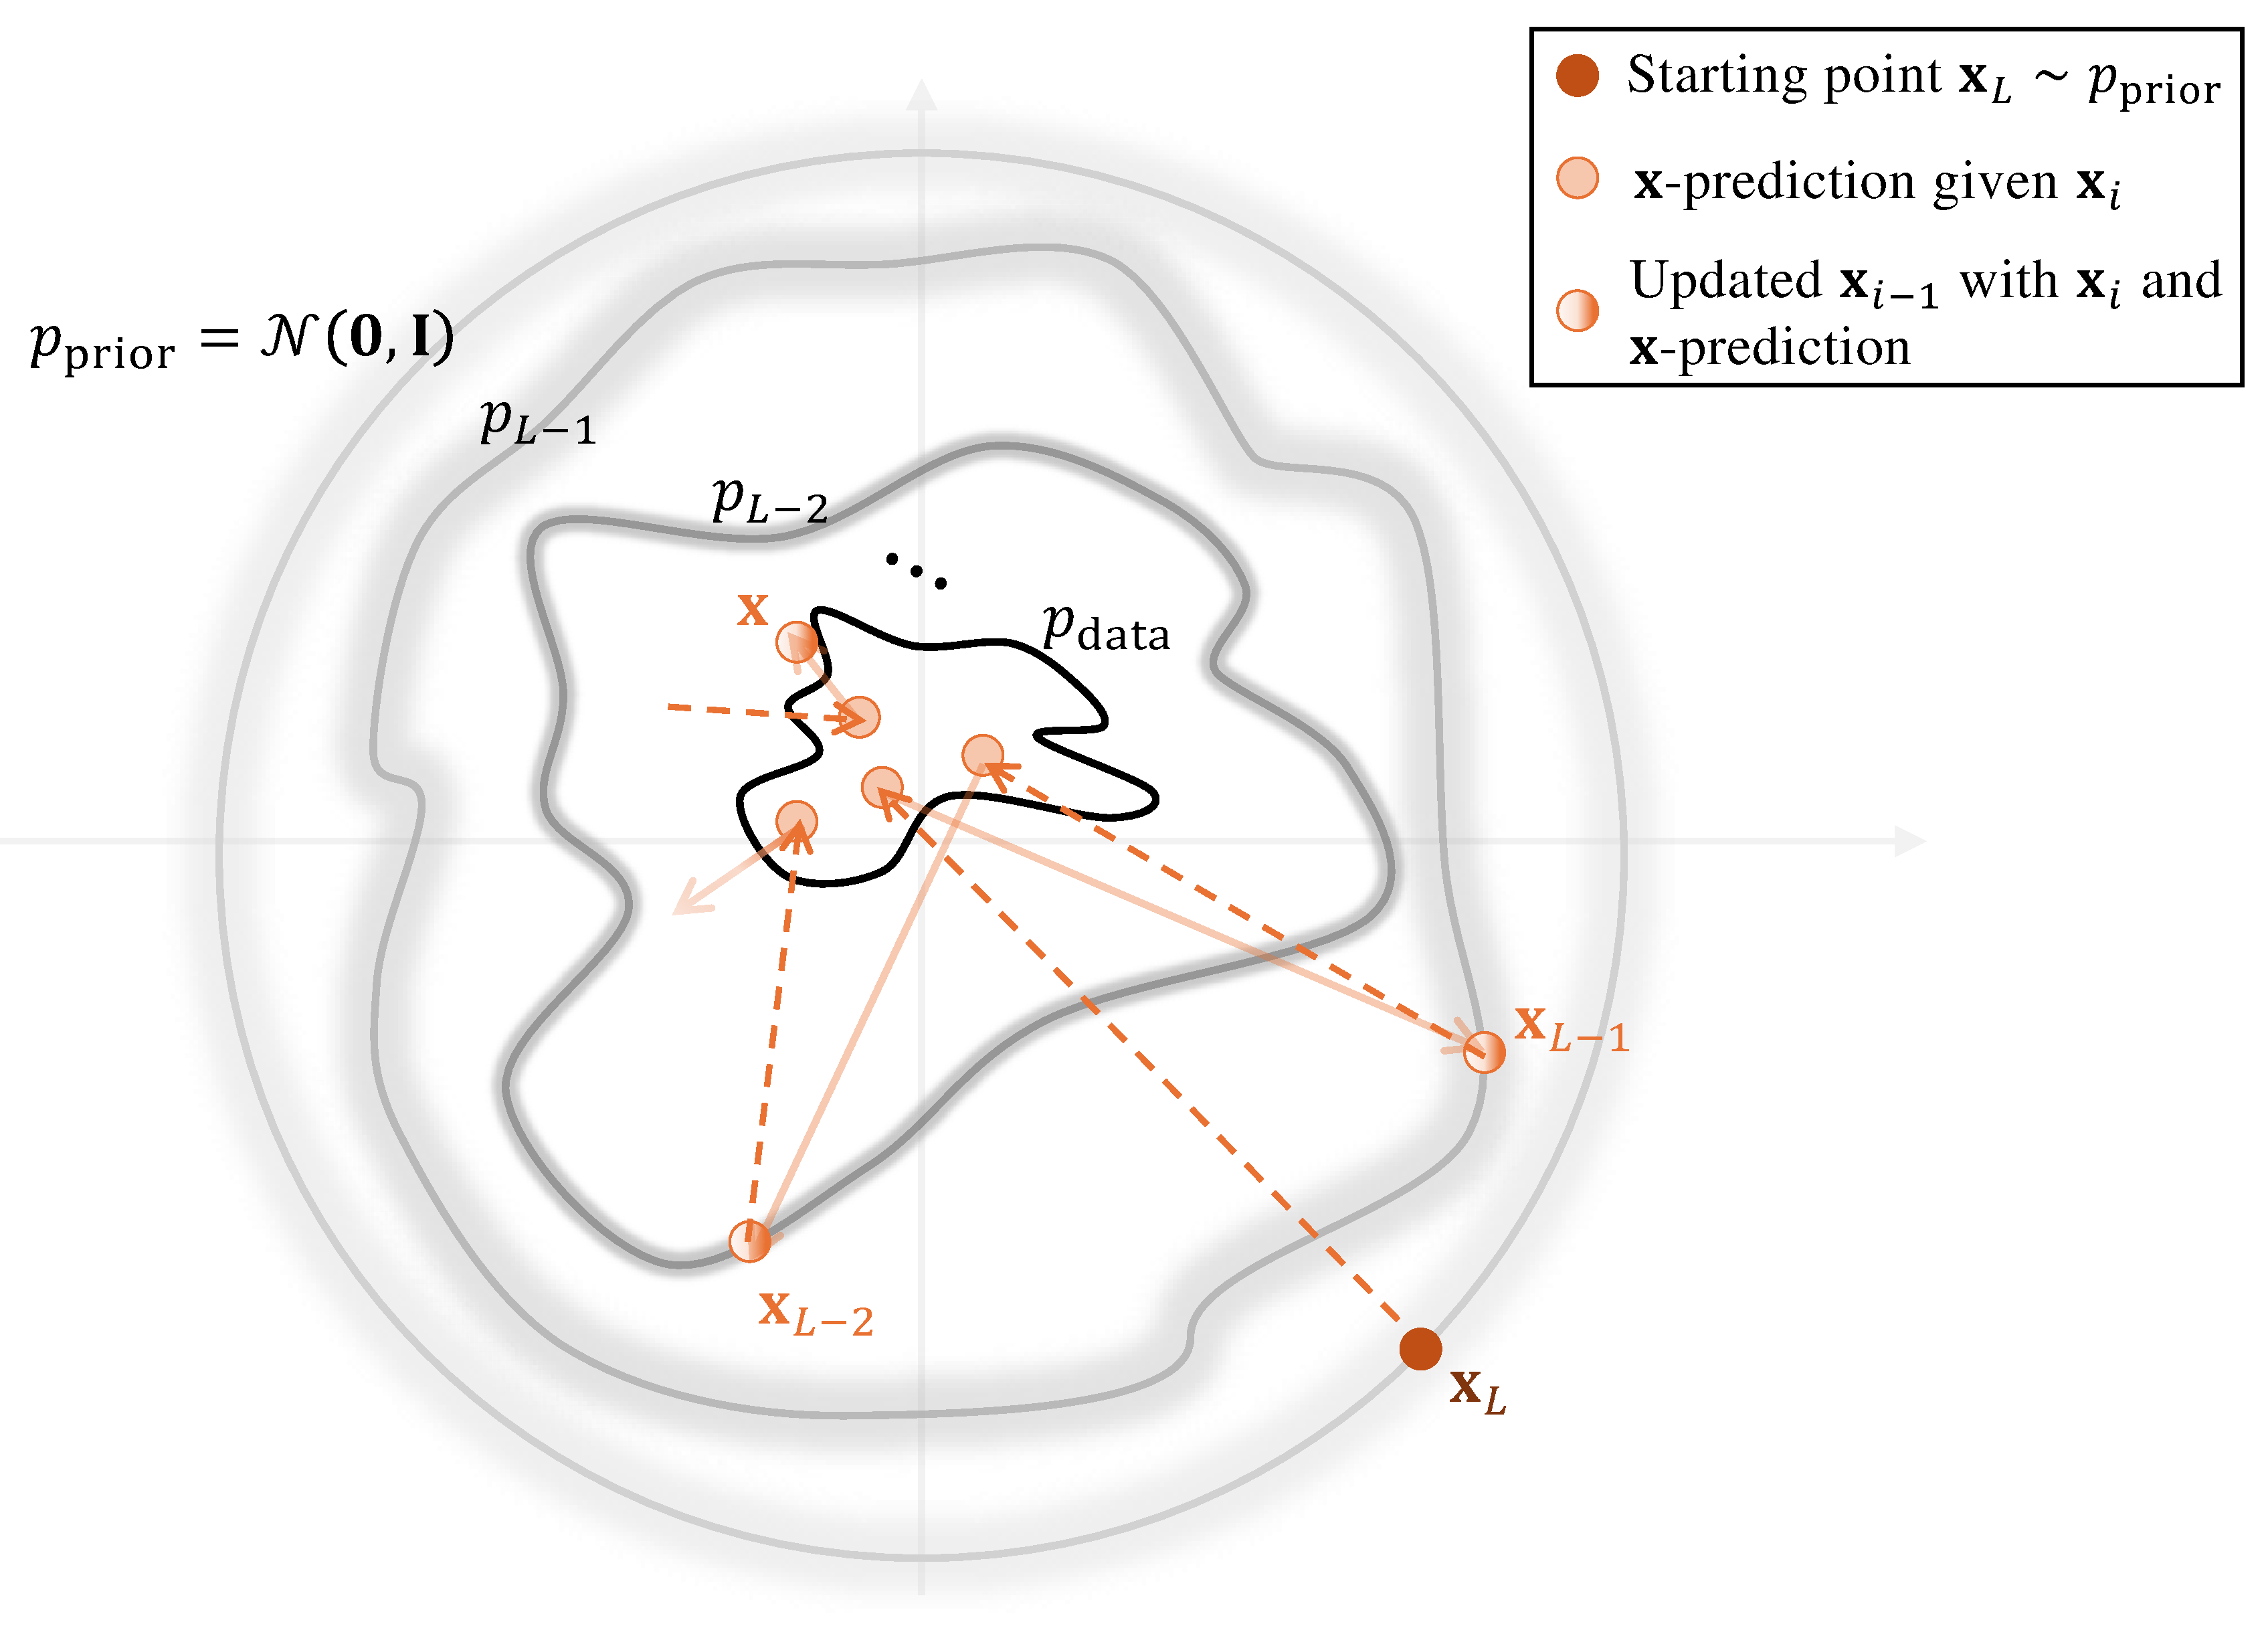
\includegraphics[width=\linewidth]{Images/PartB/diffusion-clean.pdf}
\caption{\textbfs{Illustration of the denoise-then-re-noise view of
    DDPM sampling.} From the current noisy sample $\mathbf{x}_i$, the model first estimates the underlying clean signal $\mathbf{x}_{\bm{\phi}^\times}(\mathbf{x}_i,i)$, and then samples a less noisy point $\mathbf{x}_{i-1}$ by re-noising this estimate to the $(i-1)$-th noise level. \figcredit{Created by the authors.}}
    \label{fig:vdm-clean}
\end{figure}



\paragraph{Slow Sampling Speed of DDPM.} Sampling in DDPMs (i.e., diffusion models) is inherently slow. In the original formulation and implementation, generating a sample typically requires around $1{,}000$ denoising steps. This is because sampling proceeds through a long sequence of small refinements: at each step, the model updates the current noisy sample slightly toward a cleaner one, and the next update must start from the result of the previous step. As a result, standard DDPM sampling is time-stepping and strongly sequential, and good sample quality usually requires many such steps to closely track the reverse diffusion path.

Theorem~\ref{thm:equiv-marginal-kl} shows that an expressive $ p_{\bm{\phi}}(\mathbf{x}_{i-1} | \mathbf{x}_i) $ can theoretically match the true reverse distribution $ p(\mathbf{x}_{i-1} | \mathbf{x}_i) $. However, in practice, $ p_{\bm{\phi}}(\mathbf{x}_{i-1} | \mathbf{x}_i) $ is typically modeled as a Gaussian to approximate $ p(\mathbf{x}_{i-1} | \mathbf{x}_i) $, limiting its expressiveness.

For small forward noise scales $\beta_i$, the true reverse distribution is approximately Gaussian, enabling accurate approximation. Conversely, large $\beta_i$ induce multimodality or strong non-Gaussianity that a single Gaussian cannot capture. To maintain accuracy, DDPM employs many small $\beta_i$ steps, forming a sequential chain where each step depends on the previous and requires a neural network evaluation $\boldsymbol{\epsilon}_{\bm{\phi}^\times}(\mathbf{x}_i, i)$. This results in $\mathcal{O}(L)$ sequential passes, preventing parallelization and slowing generation.



Later in \Cref{ch:score-sde} we show a more principled interpretation of this inherent sampling bottleneck as a differential-equation problem, which motivates continuous-time numerical strategies for accelerating generation.



\newpage
\section{Closing Remarks}\label{sec:ch2_cr}


In this chapter, we have traced the origins of diffusion models through the variational lens. We began with the Variational Autoencoder (VAE), a foundational generative model that learns a probabilistic mapping between data and a structured latent space via the Evidence Lower Bound (ELBO). We saw how Hierarchical VAEs (HVAEs) extended this idea by stacking latent layers, introducing the powerful concept of progressive, coarse-to-fine generation. However, these models face challenges with training stability and sample quality.





We then framed Denoising Diffusion Probabilistic Models (DDPMs) as a pivotal evolution within this variational framework. By fixing the encoder to a gradual noising process and learning only the reverse denoising steps, DDPMs elegantly sidestep the training instabilities of HVAEs. Crucially, we demonstrated that DDPMs are also trained by maximizing a variational bound on the log-likelihood, with a training objective that decomposes into a series of simple denoising tasks. This tractability is enabled by a powerful conditioning strategy that transforms an intractable marginal objective into a tractable conditional one, a recurring theme in diffusion models.





While this variational framework provides a complete and powerful foundation for DDPMs, it is not the only way to understand them. An alternative and equally fundamental perspective emerges from the principles of energy-based modeling. In the next chapter, we will explore this score-based perspective:
\begin{enumerate}
    \item We will shift our focus from learning the denoising transition probabilities $p_{\bm{\phi}}(\mathbf{x}_{i-1}\vert\mathbf{x}_{i})$ to directly learning the gradient of the data's log-density, i.e., the score function.
    \item We will see how this approach, originating from EBMs, gives rise to Noise Conditional Score Networks (NCSN) and reveals a deep, mathematical equivalence between the noise prediction ($\bm{\epsilon}$-prediction) learned in DDPMs and the score function itself.
\end{enumerate}

This alternative viewpoint will not only offer new insights but also serve as another cornerstone for the unified, continuous-time framework of diffusion models to be developed later.







